\documentclass{beamer}

\usepackage{mymetropolis}
%\usepackage{lmodern}
\usepackage{helvet}
\usefonttheme{default}
\usepackage{appendixnumberbeamer}

\usepackage{macros}
%\input{slides.tex}


\usepackage{overpic}

\newcommand{\lmbd}[1]{\SI{#1}{\nano\metre}}
\newcommand{\zr}{z_\mathsc{R}}
\newcommand{\chie}{\chi_\mathsc{eff}}
\newcommand{\dke}{\Delta k_\mathsc{eff}}
\newcommand{\alphae}[1]{\SI{#1}{\percent\per\watt}}

\title{Réalisation d'un laser à 532~nm\\ par génération de seconde harmonique}
\date{31 août 2023} %TODO
\author{Alexandre Fouquet}
%\institute{Stage de L3}


\begin{document}
\maketitle

{\metroset{sectionpage=none}
\section{Présentation du stage}
\setbeamertemplate{navigation symbols}{\normalsize\insertframenumber/\inserttotalframenumber}

\begin{frame}{}

\begin{center}
\large Stage L3
\end{center}

\begin{columns}
\column{0.65\linewidth}
Groupe Gaz quantiques \\
Laboratoire Kastler Brossel \\
Collège de France \\
Équipe Rubidium \\
%maître de stage : Jérôme Beugnon
\column{0.35\linewidth}
\vspace{-0.5cm}
\begin{figure}[htbp]
  \centering
  \includegraphics<1->[width=\textwidth]{img/logos_small_t.png}
\end{figure}
\end{columns}

\begin{center}
\large Maître de stage : Jérôme Beugnon
\end{center}

%\begin{figure}[htbp]
%  \centering
%  \includegraphics<1->[width=0.9\textwidth]{img/equipe.jpg}
%\end{figure}
\end{frame}


\begin{frame}{Obtention d'un gaz dégénéré à 2 dimensions}
\begin{columns}
\column{0.59\linewidth}
%L'équipe Rubidium travaille sur des gaz de rubidium dégénérés (``condensats'') à deux dimensions.
%
Condensats 2D de gaz de rubidium soumis à un potentiel contrôlé

\vspace{0.5cm}
À partir d'un condensat 3D, piégeage dans les zones sombres par un laser à $\lmbd{532}$ (force dipolaire) :
  \begin{itemize}%[<+->]
  \item plan : réseau optique
  \item potentiel (disque) : DMD\\(\textit{digital micromirror device})
  \end{itemize}
\column{0.41\linewidth}
%\includegraphics[height=7.5cm]{img/accordeon-dmd.png}
\begin{overpic}[percent,scale=0.35,tics=5]{img/accordeon-dmd.png}
    \put(51,79){DMD}
    \put(34,74){objectif de}
    \put(34,70){microscope}
%    \put(34,64){paroi}
\end{overpic}
\end{columns}
\end{frame}

%\begin{frame}{Piégeage par les lasers à 532~nm} %TODO
%\begin{columns}
%\column{0.7\linewidth}
%\visible<1->{%
%Force de piégeage dipolaire (polarisation de l'atome)
%\vspace*{-0.5cm}
%\begin{align*}
%&\v F_\mathsc{dip}(\v r) = - \v \nabla U_\mathsc{dip}(\v r),\,
%U_\mathsc{dip}(\v r)=\frac{3\pi c^2}{2\omega_0^3} \frac{\Gamma}{\widetilde\Delta} I(\v r) \,, \\
%&\quad\Gamma \text{ la largeur naturelle de la transition}\,, \\
%&\quad\frac{1}{\widetilde{\Delta}} = \frac1{\omega - \omega_0} + \frac{1}{\omega+\omega_0} \approx \frac1{\omega - \omega_0}\,.
%\end{align*}
%}%
%%\visible<1->{%
%%%\vspace*{0.4cm}
%%Force de pression de radiation $\v F = \hbar \v k \gamma$ avec $\gamma$ le taux d'émission spontanée 
%%%\vspace{-0.3cm}
%%\[ \gamma(\v r) =\frac{3\pi c^2}{2\hbar\omega_0^3} \left(\frac{\Gamma}{\widetilde\Delta}\right)^2 I(\v r)\,.\]
%%}%
%%\vspace*{-0.3cm}
%\visible<1->{%
%\begin{beamerboxesrounded}[width=\textwidth]{}
%Laser désaccordé vers le bleu : piégeage dans les zones sombres
%\end{beamerboxesrounded}
%}%
%\column{0.3\linewidth}
%\tikzset{every picture/.style={scale=0.8}}
%\centering
%\visible<1->{\input{img/transitions.tex}}
%\end{columns}
%\end{frame}

\begin{frame}{Objectif du stage}
\begin{itemize}
\item Lasers verts coûteux et fragiles
\item Fabriquer le laser dans le labo à partir d'un laser à $\lmbd{1064}$ plus facile d'accès
\item par doublage de fréquence (génération de seconde harmonique)
\end{itemize}
\begin{beamerboxesrounded}[width=0.9\textwidth]{}
Objectif : réalisation du laser à $\lmbd{532}$ de $\sim\SI{2}{W}$ et étude\\de l'efficacité du doublage et de sa stabilité
\end{beamerboxesrounded} %TODO
\end{frame}

}

\section{Principe de la génération}

\begin{frame}{Milieu non linéaire}
Équation d'onde dans un milieu non magnétique \only<2->{\textcolor{red}{non}} linéaire,\\ dans le domaine de Fourier (équation de Helmholtz) :
\begin{equation*}
\boldsymbol{\nabla}^2 \boldsymbol{\E}_q + \frac{\omega_q^2}{c^2}\tens\epsilon^{(1)}(\omega_q)\cdot \v \E_q(\v r) = \alt<1>{0}{{\textcolor{red}{- \frac{\omega_q^2}{\epsilon_0 c^2} \boldsymbol{\mathcal{P}}^\mathsc{NL}_q(\v r) }} }
\end{equation*}
avec $\tens \epsilon^{(1)}$ le tenseur de permittivité diélectrique relative (linéaire)\\
\only<2->{et $\boldsymbol{\mathcal{P}}^\mathsc{NL}_q$ la $q$-ème harmonique de la polarisation non-linéaire}

\pause
En particulier, $\v P^{(2)} \propto \tens\chi^{(2)} \v E^2$ avec $\tens\chi^{(2)}$ la susceptibilité d'ordre 2

%\pause
$\rightarrow$ $\v P^{(2)}_2 \propto \tens\chi^{(2)} \v E^2_1$ : terme source à la fréquence double
\end{frame}

\begin{frame}{Accord de phase (onde plane)}

\begin{figure}
\centering
%\vspace{0.2cm}
%\begin{beamerboxesrounded}[width=\textwidth]{}
%Le rayonnement généré en différents points interfère :
%\end{beamerboxesrounded}
%\vspace{-0.3cm}
%\tikzset{every picture/.style={height=5cm}}
%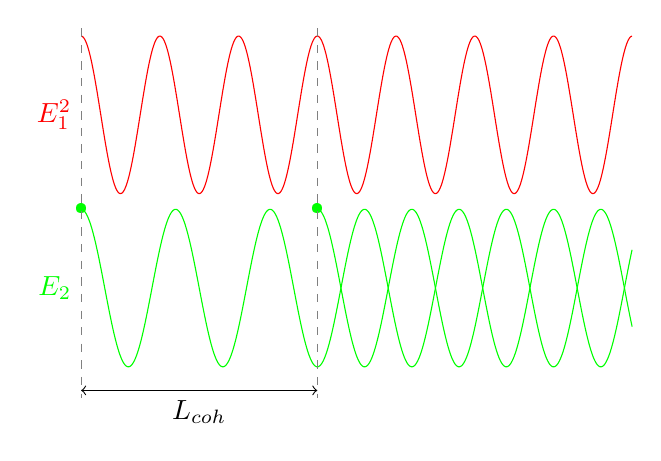
\begin{tikzpicture}[
indic/.style = {gray, dashed}
]
\def\xe{7}

%\fill[black!20] (0,1.1) rectangle (\xe,-3.3);
\draw[color=red] node[left] {$E_1^2$}  plot[samples=1000, domain=0:\xe] (\x,{cos(360* \x)});
%\draw[color=green] (0,-2.2) node[left,text width=1.7 cm] {$E_2$}  plot[samples=1000, domain=0:6] (\x,{cos(300* \x)-2.2});
\draw[color=green] (0,-2.2) node[left] {$E_2$} node at (0,-1.2) {\textbullet} plot[samples=1000, domain=0:\xe] (\x,{cos(300* \x)-2.2});
\draw[color=green] node at (3,-1.2) {\textbullet} plot[samples=1000, domain=3:\xe] (\x,{cos(300* \x + 180)-2.2});
\draw[indic] (3,1.1) -- (3,-3.6);% node {$z=L_\mathsc{coh}$};
\draw[indic] (0,1.1) -- (0,-3.6);% node {$z=0$};
\draw [<->] (0,-3.5) -- +(3,0) node[midway,below] {$L_\mathsc{coh}$};
%\draw (current bounding box.north east) rectangle (current bounding box.south west);
\end{tikzpicture}%
\includegraphics[scale=0.9]{img/accord.pdf}
\end{figure}
\vspace{-0.5cm}
Interférence destructive du rayonnement émis en 2 points distants de $L_\mathsc{coh} = \frac{\pi}{\Delta k}$ où $\Delta k = k_2 - 2 k_1 = \frac{2\pi}{\lambda_2} \left(n_2 - n_1\right)$

Accord de phase $\Delta k = 0$, $n_1 = n_2$ exclu
\end{frame}

\begin{frame}{Accord de phase (onde plane)}
\centering
% This file was created with tikzplotlib v0.10.1.
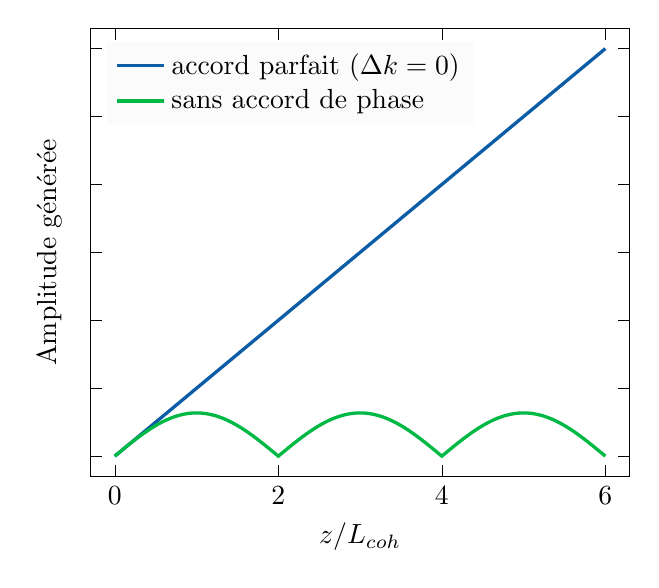
\begin{tikzpicture}

\definecolor{darkgray176}{RGB}{176,176,176}
\definecolor{darkorange2551490}{RGB}{255,149,0}
\definecolor{limegreen018569}{RGB}{0,185,69}
\definecolor{orangered255440}{RGB}{255,44,0}
\definecolor{teal1293165}{RGB}{12,93,165}

\begin{axis}[
legend cell align={left},
legend style={
	fill=black!2,
  fill opacity=0.8,
  draw opacity=1,
  text opacity=1,
  at={(0.03,0.97)},
  anchor=north west,
  draw=none
},
tick pos=both,
x grid style={darkgray176},
xlabel={\(\displaystyle z/L_\text{coh}\)},
xmin=-0.3, xmax=6.3,
xtick style={color=black},
xtick={-2,0,2,4,6,8},
xticklabels={
  \(\displaystyle {\ensuremath{-}2}\),
  \(\displaystyle {0}\),
  \(\displaystyle {2}\),
  \(\displaystyle {4}\),
  \(\displaystyle {6}\),
  \(\displaystyle {8}\)
},
y grid style={darkgray176},
ylabel={Amplitude générée},
ymin=-0.3, ymax=6.3,
ytick style={color=black},
ytick={-1,0,1,2,3,4,5,6,7},
yticklabels={
%  \(\displaystyle {\ensuremath{-}1}\),
%  \(\displaystyle {0}\),
%  \(\displaystyle {1}\),
%  \(\displaystyle {2}\),
%  \(\displaystyle {3}\),
%  \(\displaystyle {4}\),
%  \(\displaystyle {5}\),
%  \(\displaystyle {6}\),
%  \(\displaystyle {7}\)
}
]
\addplot [very thick, teal1293165]
table {%
0 0
0.00600600600600601 0.00600600600600601
0.012012012012012 0.012012012012012
0.018018018018018 0.018018018018018
0.024024024024024 0.024024024024024
0.03003003003003 0.03003003003003
0.036036036036036 0.036036036036036
0.042042042042042 0.042042042042042
0.048048048048048 0.048048048048048
0.0540540540540541 0.0540540540540541
0.0600600600600601 0.0600600600600601
0.0660660660660661 0.0660660660660661
0.0720720720720721 0.0720720720720721
0.0780780780780781 0.0780780780780781
0.0840840840840841 0.0840840840840841
0.0900900900900901 0.0900900900900901
0.0960960960960961 0.0960960960960961
0.102102102102102 0.102102102102102
0.108108108108108 0.108108108108108
0.114114114114114 0.114114114114114
0.12012012012012 0.12012012012012
0.126126126126126 0.126126126126126
0.132132132132132 0.132132132132132
0.138138138138138 0.138138138138138
0.144144144144144 0.144144144144144
0.15015015015015 0.15015015015015
0.156156156156156 0.156156156156156
0.162162162162162 0.162162162162162
0.168168168168168 0.168168168168168
0.174174174174174 0.174174174174174
0.18018018018018 0.18018018018018
0.186186186186186 0.186186186186186
0.192192192192192 0.192192192192192
0.198198198198198 0.198198198198198
0.204204204204204 0.204204204204204
0.21021021021021 0.21021021021021
0.216216216216216 0.216216216216216
0.222222222222222 0.222222222222222
0.228228228228228 0.228228228228228
0.234234234234234 0.234234234234234
0.24024024024024 0.24024024024024
0.246246246246246 0.246246246246246
0.252252252252252 0.252252252252252
0.258258258258258 0.258258258258258
0.264264264264264 0.264264264264264
0.27027027027027 0.27027027027027
0.276276276276276 0.276276276276276
0.282282282282282 0.282282282282282
0.288288288288288 0.288288288288288
0.294294294294294 0.294294294294294
0.3003003003003 0.3003003003003
0.306306306306306 0.306306306306306
0.312312312312312 0.312312312312312
0.318318318318318 0.318318318318318
0.324324324324324 0.324324324324324
0.33033033033033 0.33033033033033
0.336336336336336 0.336336336336336
0.342342342342342 0.342342342342342
0.348348348348348 0.348348348348348
0.354354354354354 0.354354354354354
0.36036036036036 0.36036036036036
0.366366366366366 0.366366366366366
0.372372372372372 0.372372372372372
0.378378378378378 0.378378378378378
0.384384384384384 0.384384384384384
0.39039039039039 0.39039039039039
0.396396396396396 0.396396396396396
0.402402402402402 0.402402402402402
0.408408408408408 0.408408408408408
0.414414414414414 0.414414414414414
0.42042042042042 0.42042042042042
0.426426426426426 0.426426426426426
0.432432432432432 0.432432432432432
0.438438438438438 0.438438438438438
0.444444444444444 0.444444444444444
0.45045045045045 0.45045045045045
0.456456456456456 0.456456456456456
0.462462462462462 0.462462462462462
0.468468468468468 0.468468468468468
0.474474474474474 0.474474474474474
0.48048048048048 0.48048048048048
0.486486486486486 0.486486486486486
0.492492492492492 0.492492492492492
0.498498498498498 0.498498498498498
0.504504504504504 0.504504504504504
0.510510510510511 0.510510510510511
0.516516516516517 0.516516516516517
0.522522522522523 0.522522522522523
0.528528528528528 0.528528528528528
0.534534534534534 0.534534534534534
0.540540540540541 0.540540540540541
0.546546546546547 0.546546546546547
0.552552552552553 0.552552552552553
0.558558558558559 0.558558558558559
0.564564564564565 0.564564564564565
0.570570570570571 0.570570570570571
0.576576576576577 0.576576576576577
0.582582582582583 0.582582582582583
0.588588588588589 0.588588588588589
0.594594594594595 0.594594594594595
0.600600600600601 0.600600600600601
0.606606606606607 0.606606606606607
0.612612612612613 0.612612612612613
0.618618618618619 0.618618618618619
0.624624624624625 0.624624624624625
0.630630630630631 0.630630630630631
0.636636636636637 0.636636636636637
0.642642642642643 0.642642642642643
0.648648648648649 0.648648648648649
0.654654654654655 0.654654654654655
0.660660660660661 0.660660660660661
0.666666666666667 0.666666666666667
0.672672672672673 0.672672672672673
0.678678678678679 0.678678678678679
0.684684684684685 0.684684684684685
0.690690690690691 0.690690690690691
0.696696696696697 0.696696696696697
0.702702702702703 0.702702702702703
0.708708708708709 0.708708708708709
0.714714714714715 0.714714714714715
0.720720720720721 0.720720720720721
0.726726726726727 0.726726726726727
0.732732732732733 0.732732732732733
0.738738738738739 0.738738738738739
0.744744744744745 0.744744744744745
0.750750750750751 0.750750750750751
0.756756756756757 0.756756756756757
0.762762762762763 0.762762762762763
0.768768768768769 0.768768768768769
0.774774774774775 0.774774774774775
0.780780780780781 0.780780780780781
0.786786786786787 0.786786786786787
0.792792792792793 0.792792792792793
0.798798798798799 0.798798798798799
0.804804804804805 0.804804804804805
0.810810810810811 0.810810810810811
0.816816816816817 0.816816816816817
0.822822822822823 0.822822822822823
0.828828828828829 0.828828828828829
0.834834834834835 0.834834834834835
0.840840840840841 0.840840840840841
0.846846846846847 0.846846846846847
0.852852852852853 0.852852852852853
0.858858858858859 0.858858858858859
0.864864864864865 0.864864864864865
0.870870870870871 0.870870870870871
0.876876876876877 0.876876876876877
0.882882882882883 0.882882882882883
0.888888888888889 0.888888888888889
0.894894894894895 0.894894894894895
0.900900900900901 0.900900900900901
0.906906906906907 0.906906906906907
0.912912912912913 0.912912912912913
0.918918918918919 0.918918918918919
0.924924924924925 0.924924924924925
0.930930930930931 0.930930930930931
0.936936936936937 0.936936936936937
0.942942942942943 0.942942942942943
0.948948948948949 0.948948948948949
0.954954954954955 0.954954954954955
0.960960960960961 0.960960960960961
0.966966966966967 0.966966966966967
0.972972972972973 0.972972972972973
0.978978978978979 0.978978978978979
0.984984984984985 0.984984984984985
0.990990990990991 0.990990990990991
0.996996996996997 0.996996996996997
1.003003003003 1.003003003003
1.00900900900901 1.00900900900901
1.01501501501502 1.01501501501502
1.02102102102102 1.02102102102102
1.02702702702703 1.02702702702703
1.03303303303303 1.03303303303303
1.03903903903904 1.03903903903904
1.04504504504505 1.04504504504505
1.05105105105105 1.05105105105105
1.05705705705706 1.05705705705706
1.06306306306306 1.06306306306306
1.06906906906907 1.06906906906907
1.07507507507508 1.07507507507508
1.08108108108108 1.08108108108108
1.08708708708709 1.08708708708709
1.09309309309309 1.09309309309309
1.0990990990991 1.0990990990991
1.10510510510511 1.10510510510511
1.11111111111111 1.11111111111111
1.11711711711712 1.11711711711712
1.12312312312312 1.12312312312312
1.12912912912913 1.12912912912913
1.13513513513514 1.13513513513514
1.14114114114114 1.14114114114114
1.14714714714715 1.14714714714715
1.15315315315315 1.15315315315315
1.15915915915916 1.15915915915916
1.16516516516517 1.16516516516517
1.17117117117117 1.17117117117117
1.17717717717718 1.17717717717718
1.18318318318318 1.18318318318318
1.18918918918919 1.18918918918919
1.1951951951952 1.1951951951952
1.2012012012012 1.2012012012012
1.20720720720721 1.20720720720721
1.21321321321321 1.21321321321321
1.21921921921922 1.21921921921922
1.22522522522523 1.22522522522523
1.23123123123123 1.23123123123123
1.23723723723724 1.23723723723724
1.24324324324324 1.24324324324324
1.24924924924925 1.24924924924925
1.25525525525526 1.25525525525526
1.26126126126126 1.26126126126126
1.26726726726727 1.26726726726727
1.27327327327327 1.27327327327327
1.27927927927928 1.27927927927928
1.28528528528529 1.28528528528529
1.29129129129129 1.29129129129129
1.2972972972973 1.2972972972973
1.3033033033033 1.3033033033033
1.30930930930931 1.30930930930931
1.31531531531532 1.31531531531532
1.32132132132132 1.32132132132132
1.32732732732733 1.32732732732733
1.33333333333333 1.33333333333333
1.33933933933934 1.33933933933934
1.34534534534535 1.34534534534535
1.35135135135135 1.35135135135135
1.35735735735736 1.35735735735736
1.36336336336336 1.36336336336336
1.36936936936937 1.36936936936937
1.37537537537538 1.37537537537538
1.38138138138138 1.38138138138138
1.38738738738739 1.38738738738739
1.39339339339339 1.39339339339339
1.3993993993994 1.3993993993994
1.40540540540541 1.40540540540541
1.41141141141141 1.41141141141141
1.41741741741742 1.41741741741742
1.42342342342342 1.42342342342342
1.42942942942943 1.42942942942943
1.43543543543544 1.43543543543544
1.44144144144144 1.44144144144144
1.44744744744745 1.44744744744745
1.45345345345345 1.45345345345345
1.45945945945946 1.45945945945946
1.46546546546547 1.46546546546547
1.47147147147147 1.47147147147147
1.47747747747748 1.47747747747748
1.48348348348348 1.48348348348348
1.48948948948949 1.48948948948949
1.4954954954955 1.4954954954955
1.5015015015015 1.5015015015015
1.50750750750751 1.50750750750751
1.51351351351351 1.51351351351351
1.51951951951952 1.51951951951952
1.52552552552553 1.52552552552553
1.53153153153153 1.53153153153153
1.53753753753754 1.53753753753754
1.54354354354354 1.54354354354354
1.54954954954955 1.54954954954955
1.55555555555556 1.55555555555556
1.56156156156156 1.56156156156156
1.56756756756757 1.56756756756757
1.57357357357357 1.57357357357357
1.57957957957958 1.57957957957958
1.58558558558559 1.58558558558559
1.59159159159159 1.59159159159159
1.5975975975976 1.5975975975976
1.6036036036036 1.6036036036036
1.60960960960961 1.60960960960961
1.61561561561562 1.61561561561562
1.62162162162162 1.62162162162162
1.62762762762763 1.62762762762763
1.63363363363363 1.63363363363363
1.63963963963964 1.63963963963964
1.64564564564565 1.64564564564565
1.65165165165165 1.65165165165165
1.65765765765766 1.65765765765766
1.66366366366366 1.66366366366366
1.66966966966967 1.66966966966967
1.67567567567568 1.67567567567568
1.68168168168168 1.68168168168168
1.68768768768769 1.68768768768769
1.69369369369369 1.69369369369369
1.6996996996997 1.6996996996997
1.70570570570571 1.70570570570571
1.71171171171171 1.71171171171171
1.71771771771772 1.71771771771772
1.72372372372372 1.72372372372372
1.72972972972973 1.72972972972973
1.73573573573574 1.73573573573574
1.74174174174174 1.74174174174174
1.74774774774775 1.74774774774775
1.75375375375375 1.75375375375375
1.75975975975976 1.75975975975976
1.76576576576577 1.76576576576577
1.77177177177177 1.77177177177177
1.77777777777778 1.77777777777778
1.78378378378378 1.78378378378378
1.78978978978979 1.78978978978979
1.7957957957958 1.7957957957958
1.8018018018018 1.8018018018018
1.80780780780781 1.80780780780781
1.81381381381381 1.81381381381381
1.81981981981982 1.81981981981982
1.82582582582583 1.82582582582583
1.83183183183183 1.83183183183183
1.83783783783784 1.83783783783784
1.84384384384384 1.84384384384384
1.84984984984985 1.84984984984985
1.85585585585586 1.85585585585586
1.86186186186186 1.86186186186186
1.86786786786787 1.86786786786787
1.87387387387387 1.87387387387387
1.87987987987988 1.87987987987988
1.88588588588589 1.88588588588589
1.89189189189189 1.89189189189189
1.8978978978979 1.8978978978979
1.9039039039039 1.9039039039039
1.90990990990991 1.90990990990991
1.91591591591592 1.91591591591592
1.92192192192192 1.92192192192192
1.92792792792793 1.92792792792793
1.93393393393393 1.93393393393393
1.93993993993994 1.93993993993994
1.94594594594595 1.94594594594595
1.95195195195195 1.95195195195195
1.95795795795796 1.95795795795796
1.96396396396396 1.96396396396396
1.96996996996997 1.96996996996997
1.97597597597598 1.97597597597598
1.98198198198198 1.98198198198198
1.98798798798799 1.98798798798799
1.99399399399399 1.99399399399399
2 2
2.00600600600601 2.00600600600601
2.01201201201201 2.01201201201201
2.01801801801802 2.01801801801802
2.02402402402402 2.02402402402402
2.03003003003003 2.03003003003003
2.03603603603604 2.03603603603604
2.04204204204204 2.04204204204204
2.04804804804805 2.04804804804805
2.05405405405405 2.05405405405405
2.06006006006006 2.06006006006006
2.06606606606607 2.06606606606607
2.07207207207207 2.07207207207207
2.07807807807808 2.07807807807808
2.08408408408408 2.08408408408408
2.09009009009009 2.09009009009009
2.0960960960961 2.0960960960961
2.1021021021021 2.1021021021021
2.10810810810811 2.10810810810811
2.11411411411411 2.11411411411411
2.12012012012012 2.12012012012012
2.12612612612613 2.12612612612613
2.13213213213213 2.13213213213213
2.13813813813814 2.13813813813814
2.14414414414414 2.14414414414414
2.15015015015015 2.15015015015015
2.15615615615616 2.15615615615616
2.16216216216216 2.16216216216216
2.16816816816817 2.16816816816817
2.17417417417417 2.17417417417417
2.18018018018018 2.18018018018018
2.18618618618619 2.18618618618619
2.19219219219219 2.19219219219219
2.1981981981982 2.1981981981982
2.2042042042042 2.2042042042042
2.21021021021021 2.21021021021021
2.21621621621622 2.21621621621622
2.22222222222222 2.22222222222222
2.22822822822823 2.22822822822823
2.23423423423423 2.23423423423423
2.24024024024024 2.24024024024024
2.24624624624625 2.24624624624625
2.25225225225225 2.25225225225225
2.25825825825826 2.25825825825826
2.26426426426426 2.26426426426426
2.27027027027027 2.27027027027027
2.27627627627628 2.27627627627628
2.28228228228228 2.28228228228228
2.28828828828829 2.28828828828829
2.29429429429429 2.29429429429429
2.3003003003003 2.3003003003003
2.30630630630631 2.30630630630631
2.31231231231231 2.31231231231231
2.31831831831832 2.31831831831832
2.32432432432432 2.32432432432432
2.33033033033033 2.33033033033033
2.33633633633634 2.33633633633634
2.34234234234234 2.34234234234234
2.34834834834835 2.34834834834835
2.35435435435435 2.35435435435435
2.36036036036036 2.36036036036036
2.36636636636637 2.36636636636637
2.37237237237237 2.37237237237237
2.37837837837838 2.37837837837838
2.38438438438438 2.38438438438438
2.39039039039039 2.39039039039039
2.3963963963964 2.3963963963964
2.4024024024024 2.4024024024024
2.40840840840841 2.40840840840841
2.41441441441441 2.41441441441441
2.42042042042042 2.42042042042042
2.42642642642643 2.42642642642643
2.43243243243243 2.43243243243243
2.43843843843844 2.43843843843844
2.44444444444444 2.44444444444444
2.45045045045045 2.45045045045045
2.45645645645646 2.45645645645646
2.46246246246246 2.46246246246246
2.46846846846847 2.46846846846847
2.47447447447447 2.47447447447447
2.48048048048048 2.48048048048048
2.48648648648649 2.48648648648649
2.49249249249249 2.49249249249249
2.4984984984985 2.4984984984985
2.5045045045045 2.5045045045045
2.51051051051051 2.51051051051051
2.51651651651652 2.51651651651652
2.52252252252252 2.52252252252252
2.52852852852853 2.52852852852853
2.53453453453453 2.53453453453453
2.54054054054054 2.54054054054054
2.54654654654655 2.54654654654655
2.55255255255255 2.55255255255255
2.55855855855856 2.55855855855856
2.56456456456456 2.56456456456456
2.57057057057057 2.57057057057057
2.57657657657658 2.57657657657658
2.58258258258258 2.58258258258258
2.58858858858859 2.58858858858859
2.59459459459459 2.59459459459459
2.6006006006006 2.6006006006006
2.60660660660661 2.60660660660661
2.61261261261261 2.61261261261261
2.61861861861862 2.61861861861862
2.62462462462462 2.62462462462462
2.63063063063063 2.63063063063063
2.63663663663664 2.63663663663664
2.64264264264264 2.64264264264264
2.64864864864865 2.64864864864865
2.65465465465465 2.65465465465465
2.66066066066066 2.66066066066066
2.66666666666667 2.66666666666667
2.67267267267267 2.67267267267267
2.67867867867868 2.67867867867868
2.68468468468468 2.68468468468468
2.69069069069069 2.69069069069069
2.6966966966967 2.6966966966967
2.7027027027027 2.7027027027027
2.70870870870871 2.70870870870871
2.71471471471471 2.71471471471471
2.72072072072072 2.72072072072072
2.72672672672673 2.72672672672673
2.73273273273273 2.73273273273273
2.73873873873874 2.73873873873874
2.74474474474474 2.74474474474474
2.75075075075075 2.75075075075075
2.75675675675676 2.75675675675676
2.76276276276276 2.76276276276276
2.76876876876877 2.76876876876877
2.77477477477477 2.77477477477477
2.78078078078078 2.78078078078078
2.78678678678679 2.78678678678679
2.79279279279279 2.79279279279279
2.7987987987988 2.7987987987988
2.8048048048048 2.8048048048048
2.81081081081081 2.81081081081081
2.81681681681682 2.81681681681682
2.82282282282282 2.82282282282282
2.82882882882883 2.82882882882883
2.83483483483483 2.83483483483483
2.84084084084084 2.84084084084084
2.84684684684685 2.84684684684685
2.85285285285285 2.85285285285285
2.85885885885886 2.85885885885886
2.86486486486486 2.86486486486486
2.87087087087087 2.87087087087087
2.87687687687688 2.87687687687688
2.88288288288288 2.88288288288288
2.88888888888889 2.88888888888889
2.89489489489489 2.89489489489489
2.9009009009009 2.9009009009009
2.90690690690691 2.90690690690691
2.91291291291291 2.91291291291291
2.91891891891892 2.91891891891892
2.92492492492492 2.92492492492492
2.93093093093093 2.93093093093093
2.93693693693694 2.93693693693694
2.94294294294294 2.94294294294294
2.94894894894895 2.94894894894895
2.95495495495495 2.95495495495495
2.96096096096096 2.96096096096096
2.96696696696697 2.96696696696697
2.97297297297297 2.97297297297297
2.97897897897898 2.97897897897898
2.98498498498498 2.98498498498498
2.99099099099099 2.99099099099099
2.996996996997 2.996996996997
3.003003003003 3.003003003003
3.00900900900901 3.00900900900901
3.01501501501502 3.01501501501502
3.02102102102102 3.02102102102102
3.02702702702703 3.02702702702703
3.03303303303303 3.03303303303303
3.03903903903904 3.03903903903904
3.04504504504505 3.04504504504505
3.05105105105105 3.05105105105105
3.05705705705706 3.05705705705706
3.06306306306306 3.06306306306306
3.06906906906907 3.06906906906907
3.07507507507508 3.07507507507508
3.08108108108108 3.08108108108108
3.08708708708709 3.08708708708709
3.09309309309309 3.09309309309309
3.0990990990991 3.0990990990991
3.10510510510511 3.10510510510511
3.11111111111111 3.11111111111111
3.11711711711712 3.11711711711712
3.12312312312312 3.12312312312312
3.12912912912913 3.12912912912913
3.13513513513514 3.13513513513514
3.14114114114114 3.14114114114114
3.14714714714715 3.14714714714715
3.15315315315315 3.15315315315315
3.15915915915916 3.15915915915916
3.16516516516517 3.16516516516517
3.17117117117117 3.17117117117117
3.17717717717718 3.17717717717718
3.18318318318318 3.18318318318318
3.18918918918919 3.18918918918919
3.1951951951952 3.1951951951952
3.2012012012012 3.2012012012012
3.20720720720721 3.20720720720721
3.21321321321321 3.21321321321321
3.21921921921922 3.21921921921922
3.22522522522523 3.22522522522523
3.23123123123123 3.23123123123123
3.23723723723724 3.23723723723724
3.24324324324324 3.24324324324324
3.24924924924925 3.24924924924925
3.25525525525526 3.25525525525526
3.26126126126126 3.26126126126126
3.26726726726727 3.26726726726727
3.27327327327327 3.27327327327327
3.27927927927928 3.27927927927928
3.28528528528529 3.28528528528529
3.29129129129129 3.29129129129129
3.2972972972973 3.2972972972973
3.3033033033033 3.3033033033033
3.30930930930931 3.30930930930931
3.31531531531532 3.31531531531532
3.32132132132132 3.32132132132132
3.32732732732733 3.32732732732733
3.33333333333333 3.33333333333333
3.33933933933934 3.33933933933934
3.34534534534535 3.34534534534535
3.35135135135135 3.35135135135135
3.35735735735736 3.35735735735736
3.36336336336336 3.36336336336336
3.36936936936937 3.36936936936937
3.37537537537538 3.37537537537538
3.38138138138138 3.38138138138138
3.38738738738739 3.38738738738739
3.39339339339339 3.39339339339339
3.3993993993994 3.3993993993994
3.40540540540541 3.40540540540541
3.41141141141141 3.41141141141141
3.41741741741742 3.41741741741742
3.42342342342342 3.42342342342342
3.42942942942943 3.42942942942943
3.43543543543544 3.43543543543544
3.44144144144144 3.44144144144144
3.44744744744745 3.44744744744745
3.45345345345345 3.45345345345345
3.45945945945946 3.45945945945946
3.46546546546547 3.46546546546547
3.47147147147147 3.47147147147147
3.47747747747748 3.47747747747748
3.48348348348348 3.48348348348348
3.48948948948949 3.48948948948949
3.4954954954955 3.4954954954955
3.5015015015015 3.5015015015015
3.50750750750751 3.50750750750751
3.51351351351351 3.51351351351351
3.51951951951952 3.51951951951952
3.52552552552553 3.52552552552553
3.53153153153153 3.53153153153153
3.53753753753754 3.53753753753754
3.54354354354354 3.54354354354354
3.54954954954955 3.54954954954955
3.55555555555556 3.55555555555556
3.56156156156156 3.56156156156156
3.56756756756757 3.56756756756757
3.57357357357357 3.57357357357357
3.57957957957958 3.57957957957958
3.58558558558559 3.58558558558559
3.59159159159159 3.59159159159159
3.5975975975976 3.5975975975976
3.6036036036036 3.6036036036036
3.60960960960961 3.60960960960961
3.61561561561562 3.61561561561562
3.62162162162162 3.62162162162162
3.62762762762763 3.62762762762763
3.63363363363363 3.63363363363363
3.63963963963964 3.63963963963964
3.64564564564565 3.64564564564565
3.65165165165165 3.65165165165165
3.65765765765766 3.65765765765766
3.66366366366366 3.66366366366366
3.66966966966967 3.66966966966967
3.67567567567568 3.67567567567568
3.68168168168168 3.68168168168168
3.68768768768769 3.68768768768769
3.69369369369369 3.69369369369369
3.6996996996997 3.6996996996997
3.70570570570571 3.70570570570571
3.71171171171171 3.71171171171171
3.71771771771772 3.71771771771772
3.72372372372372 3.72372372372372
3.72972972972973 3.72972972972973
3.73573573573574 3.73573573573574
3.74174174174174 3.74174174174174
3.74774774774775 3.74774774774775
3.75375375375375 3.75375375375375
3.75975975975976 3.75975975975976
3.76576576576577 3.76576576576577
3.77177177177177 3.77177177177177
3.77777777777778 3.77777777777778
3.78378378378378 3.78378378378378
3.78978978978979 3.78978978978979
3.7957957957958 3.7957957957958
3.8018018018018 3.8018018018018
3.80780780780781 3.80780780780781
3.81381381381381 3.81381381381381
3.81981981981982 3.81981981981982
3.82582582582583 3.82582582582583
3.83183183183183 3.83183183183183
3.83783783783784 3.83783783783784
3.84384384384384 3.84384384384384
3.84984984984985 3.84984984984985
3.85585585585586 3.85585585585586
3.86186186186186 3.86186186186186
3.86786786786787 3.86786786786787
3.87387387387387 3.87387387387387
3.87987987987988 3.87987987987988
3.88588588588589 3.88588588588589
3.89189189189189 3.89189189189189
3.8978978978979 3.8978978978979
3.9039039039039 3.9039039039039
3.90990990990991 3.90990990990991
3.91591591591592 3.91591591591592
3.92192192192192 3.92192192192192
3.92792792792793 3.92792792792793
3.93393393393393 3.93393393393393
3.93993993993994 3.93993993993994
3.94594594594595 3.94594594594595
3.95195195195195 3.95195195195195
3.95795795795796 3.95795795795796
3.96396396396396 3.96396396396396
3.96996996996997 3.96996996996997
3.97597597597598 3.97597597597598
3.98198198198198 3.98198198198198
3.98798798798799 3.98798798798799
3.99399399399399 3.99399399399399
4 4
4.00600600600601 4.00600600600601
4.01201201201201 4.01201201201201
4.01801801801802 4.01801801801802
4.02402402402402 4.02402402402402
4.03003003003003 4.03003003003003
4.03603603603604 4.03603603603604
4.04204204204204 4.04204204204204
4.04804804804805 4.04804804804805
4.05405405405405 4.05405405405405
4.06006006006006 4.06006006006006
4.06606606606607 4.06606606606607
4.07207207207207 4.07207207207207
4.07807807807808 4.07807807807808
4.08408408408408 4.08408408408408
4.09009009009009 4.09009009009009
4.0960960960961 4.0960960960961
4.1021021021021 4.1021021021021
4.10810810810811 4.10810810810811
4.11411411411411 4.11411411411411
4.12012012012012 4.12012012012012
4.12612612612613 4.12612612612613
4.13213213213213 4.13213213213213
4.13813813813814 4.13813813813814
4.14414414414414 4.14414414414414
4.15015015015015 4.15015015015015
4.15615615615616 4.15615615615616
4.16216216216216 4.16216216216216
4.16816816816817 4.16816816816817
4.17417417417417 4.17417417417417
4.18018018018018 4.18018018018018
4.18618618618619 4.18618618618619
4.19219219219219 4.19219219219219
4.1981981981982 4.1981981981982
4.2042042042042 4.2042042042042
4.21021021021021 4.21021021021021
4.21621621621622 4.21621621621622
4.22222222222222 4.22222222222222
4.22822822822823 4.22822822822823
4.23423423423423 4.23423423423423
4.24024024024024 4.24024024024024
4.24624624624625 4.24624624624625
4.25225225225225 4.25225225225225
4.25825825825826 4.25825825825826
4.26426426426426 4.26426426426426
4.27027027027027 4.27027027027027
4.27627627627628 4.27627627627628
4.28228228228228 4.28228228228228
4.28828828828829 4.28828828828829
4.29429429429429 4.29429429429429
4.3003003003003 4.3003003003003
4.30630630630631 4.30630630630631
4.31231231231231 4.31231231231231
4.31831831831832 4.31831831831832
4.32432432432432 4.32432432432432
4.33033033033033 4.33033033033033
4.33633633633634 4.33633633633634
4.34234234234234 4.34234234234234
4.34834834834835 4.34834834834835
4.35435435435435 4.35435435435435
4.36036036036036 4.36036036036036
4.36636636636637 4.36636636636637
4.37237237237237 4.37237237237237
4.37837837837838 4.37837837837838
4.38438438438438 4.38438438438438
4.39039039039039 4.39039039039039
4.3963963963964 4.3963963963964
4.4024024024024 4.4024024024024
4.40840840840841 4.40840840840841
4.41441441441441 4.41441441441441
4.42042042042042 4.42042042042042
4.42642642642643 4.42642642642643
4.43243243243243 4.43243243243243
4.43843843843844 4.43843843843844
4.44444444444444 4.44444444444444
4.45045045045045 4.45045045045045
4.45645645645646 4.45645645645646
4.46246246246246 4.46246246246246
4.46846846846847 4.46846846846847
4.47447447447447 4.47447447447447
4.48048048048048 4.48048048048048
4.48648648648649 4.48648648648649
4.49249249249249 4.49249249249249
4.4984984984985 4.4984984984985
4.5045045045045 4.5045045045045
4.51051051051051 4.51051051051051
4.51651651651652 4.51651651651652
4.52252252252252 4.52252252252252
4.52852852852853 4.52852852852853
4.53453453453453 4.53453453453453
4.54054054054054 4.54054054054054
4.54654654654655 4.54654654654655
4.55255255255255 4.55255255255255
4.55855855855856 4.55855855855856
4.56456456456456 4.56456456456456
4.57057057057057 4.57057057057057
4.57657657657658 4.57657657657658
4.58258258258258 4.58258258258258
4.58858858858859 4.58858858858859
4.59459459459459 4.59459459459459
4.6006006006006 4.6006006006006
4.60660660660661 4.60660660660661
4.61261261261261 4.61261261261261
4.61861861861862 4.61861861861862
4.62462462462462 4.62462462462462
4.63063063063063 4.63063063063063
4.63663663663664 4.63663663663664
4.64264264264264 4.64264264264264
4.64864864864865 4.64864864864865
4.65465465465465 4.65465465465465
4.66066066066066 4.66066066066066
4.66666666666667 4.66666666666667
4.67267267267267 4.67267267267267
4.67867867867868 4.67867867867868
4.68468468468468 4.68468468468468
4.69069069069069 4.69069069069069
4.6966966966967 4.6966966966967
4.7027027027027 4.7027027027027
4.70870870870871 4.70870870870871
4.71471471471471 4.71471471471471
4.72072072072072 4.72072072072072
4.72672672672673 4.72672672672673
4.73273273273273 4.73273273273273
4.73873873873874 4.73873873873874
4.74474474474474 4.74474474474474
4.75075075075075 4.75075075075075
4.75675675675676 4.75675675675676
4.76276276276276 4.76276276276276
4.76876876876877 4.76876876876877
4.77477477477477 4.77477477477477
4.78078078078078 4.78078078078078
4.78678678678679 4.78678678678679
4.79279279279279 4.79279279279279
4.7987987987988 4.7987987987988
4.8048048048048 4.8048048048048
4.81081081081081 4.81081081081081
4.81681681681682 4.81681681681682
4.82282282282282 4.82282282282282
4.82882882882883 4.82882882882883
4.83483483483483 4.83483483483483
4.84084084084084 4.84084084084084
4.84684684684685 4.84684684684685
4.85285285285285 4.85285285285285
4.85885885885886 4.85885885885886
4.86486486486486 4.86486486486486
4.87087087087087 4.87087087087087
4.87687687687688 4.87687687687688
4.88288288288288 4.88288288288288
4.88888888888889 4.88888888888889
4.89489489489489 4.89489489489489
4.9009009009009 4.9009009009009
4.90690690690691 4.90690690690691
4.91291291291291 4.91291291291291
4.91891891891892 4.91891891891892
4.92492492492492 4.92492492492492
4.93093093093093 4.93093093093093
4.93693693693694 4.93693693693694
4.94294294294294 4.94294294294294
4.94894894894895 4.94894894894895
4.95495495495495 4.95495495495495
4.96096096096096 4.96096096096096
4.96696696696697 4.96696696696697
4.97297297297297 4.97297297297297
4.97897897897898 4.97897897897898
4.98498498498498 4.98498498498498
4.99099099099099 4.99099099099099
4.996996996997 4.996996996997
5.003003003003 5.003003003003
5.00900900900901 5.00900900900901
5.01501501501502 5.01501501501502
5.02102102102102 5.02102102102102
5.02702702702703 5.02702702702703
5.03303303303303 5.03303303303303
5.03903903903904 5.03903903903904
5.04504504504505 5.04504504504505
5.05105105105105 5.05105105105105
5.05705705705706 5.05705705705706
5.06306306306306 5.06306306306306
5.06906906906907 5.06906906906907
5.07507507507508 5.07507507507508
5.08108108108108 5.08108108108108
5.08708708708709 5.08708708708709
5.09309309309309 5.09309309309309
5.0990990990991 5.0990990990991
5.10510510510511 5.10510510510511
5.11111111111111 5.11111111111111
5.11711711711712 5.11711711711712
5.12312312312312 5.12312312312312
5.12912912912913 5.12912912912913
5.13513513513514 5.13513513513514
5.14114114114114 5.14114114114114
5.14714714714715 5.14714714714715
5.15315315315315 5.15315315315315
5.15915915915916 5.15915915915916
5.16516516516517 5.16516516516517
5.17117117117117 5.17117117117117
5.17717717717718 5.17717717717718
5.18318318318318 5.18318318318318
5.18918918918919 5.18918918918919
5.1951951951952 5.1951951951952
5.2012012012012 5.2012012012012
5.20720720720721 5.20720720720721
5.21321321321321 5.21321321321321
5.21921921921922 5.21921921921922
5.22522522522523 5.22522522522523
5.23123123123123 5.23123123123123
5.23723723723724 5.23723723723724
5.24324324324324 5.24324324324324
5.24924924924925 5.24924924924925
5.25525525525526 5.25525525525526
5.26126126126126 5.26126126126126
5.26726726726727 5.26726726726727
5.27327327327327 5.27327327327327
5.27927927927928 5.27927927927928
5.28528528528529 5.28528528528529
5.29129129129129 5.29129129129129
5.2972972972973 5.2972972972973
5.3033033033033 5.3033033033033
5.30930930930931 5.30930930930931
5.31531531531532 5.31531531531532
5.32132132132132 5.32132132132132
5.32732732732733 5.32732732732733
5.33333333333333 5.33333333333333
5.33933933933934 5.33933933933934
5.34534534534535 5.34534534534535
5.35135135135135 5.35135135135135
5.35735735735736 5.35735735735736
5.36336336336336 5.36336336336336
5.36936936936937 5.36936936936937
5.37537537537538 5.37537537537538
5.38138138138138 5.38138138138138
5.38738738738739 5.38738738738739
5.39339339339339 5.39339339339339
5.3993993993994 5.3993993993994
5.40540540540541 5.40540540540541
5.41141141141141 5.41141141141141
5.41741741741742 5.41741741741742
5.42342342342342 5.42342342342342
5.42942942942943 5.42942942942943
5.43543543543544 5.43543543543544
5.44144144144144 5.44144144144144
5.44744744744745 5.44744744744745
5.45345345345345 5.45345345345345
5.45945945945946 5.45945945945946
5.46546546546547 5.46546546546547
5.47147147147147 5.47147147147147
5.47747747747748 5.47747747747748
5.48348348348348 5.48348348348348
5.48948948948949 5.48948948948949
5.4954954954955 5.4954954954955
5.5015015015015 5.5015015015015
5.50750750750751 5.50750750750751
5.51351351351351 5.51351351351351
5.51951951951952 5.51951951951952
5.52552552552553 5.52552552552553
5.53153153153153 5.53153153153153
5.53753753753754 5.53753753753754
5.54354354354354 5.54354354354354
5.54954954954955 5.54954954954955
5.55555555555556 5.55555555555556
5.56156156156156 5.56156156156156
5.56756756756757 5.56756756756757
5.57357357357357 5.57357357357357
5.57957957957958 5.57957957957958
5.58558558558559 5.58558558558559
5.59159159159159 5.59159159159159
5.5975975975976 5.5975975975976
5.6036036036036 5.6036036036036
5.60960960960961 5.60960960960961
5.61561561561562 5.61561561561562
5.62162162162162 5.62162162162162
5.62762762762763 5.62762762762763
5.63363363363363 5.63363363363363
5.63963963963964 5.63963963963964
5.64564564564565 5.64564564564565
5.65165165165165 5.65165165165165
5.65765765765766 5.65765765765766
5.66366366366366 5.66366366366366
5.66966966966967 5.66966966966967
5.67567567567568 5.67567567567568
5.68168168168168 5.68168168168168
5.68768768768769 5.68768768768769
5.69369369369369 5.69369369369369
5.6996996996997 5.6996996996997
5.70570570570571 5.70570570570571
5.71171171171171 5.71171171171171
5.71771771771772 5.71771771771772
5.72372372372372 5.72372372372372
5.72972972972973 5.72972972972973
5.73573573573574 5.73573573573574
5.74174174174174 5.74174174174174
5.74774774774775 5.74774774774775
5.75375375375375 5.75375375375375
5.75975975975976 5.75975975975976
5.76576576576577 5.76576576576577
5.77177177177177 5.77177177177177
5.77777777777778 5.77777777777778
5.78378378378378 5.78378378378378
5.78978978978979 5.78978978978979
5.7957957957958 5.7957957957958
5.8018018018018 5.8018018018018
5.80780780780781 5.80780780780781
5.81381381381381 5.81381381381381
5.81981981981982 5.81981981981982
5.82582582582583 5.82582582582583
5.83183183183183 5.83183183183183
5.83783783783784 5.83783783783784
5.84384384384384 5.84384384384384
5.84984984984985 5.84984984984985
5.85585585585586 5.85585585585586
5.86186186186186 5.86186186186186
5.86786786786787 5.86786786786787
5.87387387387387 5.87387387387387
5.87987987987988 5.87987987987988
5.88588588588589 5.88588588588589
5.89189189189189 5.89189189189189
5.8978978978979 5.8978978978979
5.9039039039039 5.9039039039039
5.90990990990991 5.90990990990991
5.91591591591592 5.91591591591592
5.92192192192192 5.92192192192192
5.92792792792793 5.92792792792793
5.93393393393393 5.93393393393393
5.93993993993994 5.93993993993994
5.94594594594595 5.94594594594595
5.95195195195195 5.95195195195195
5.95795795795796 5.95795795795796
5.96396396396396 5.96396396396396
5.96996996996997 5.96996996996997
5.97597597597598 5.97597597597598
5.98198198198198 5.98198198198198
5.98798798798799 5.98798798798799
5.99399399399399 5.99399399399399
6 6
};
\addlegendentry{accord parfait ($\Delta k = 0$)}
\addplot [very thick, limegreen018569]
table {%
0 0
0.00600600600600601 0.0060057387276301
0.012012012012012 0.0120109429222971
0.018018018018018 0.0180150780986135
0.024024024024024 0.0240176098663381
0.03003003003003 0.0300180039779391
0.036036036036036 0.0360157263761442
0.042042042042042 0.0420102432414732
0.048048048048048 0.0480010210397504
0.0540540540540541 0.0539875265695907
0.0600600600600601 0.0599692270098568
0.0660660660660661 0.0659455899670822
0.0720720720720721 0.0719160835228561
0.0780780780780781 0.077880176281166
0.0840840840840841 0.0838373374156943
0.0900900900900901 0.0897870367170633
0.0960960960960961 0.0957287446400263
0.102102102102102 0.101661932350599
0.108108108108108 0.107586071773126
0.114114114114114 0.113500635637286
0.12012012012012 0.119405097525015
0.126126126126126 0.125298931917363
0.132132132132132 0.131181614241268
0.138138138138138 0.137052620916241
0.144144144144144 0.142911429400971
0.15015015015015 0.148757518239829
0.156156156156156 0.154590367109283
0.162162162162162 0.160409456864207
0.168168168168168 0.166214269584087
0.174174174174174 0.172004288619118
0.18018018018018 0.177778998636187
0.186186186186186 0.183537885664742
0.192192192192192 0.189280437142533
0.198198198198198 0.195006141961236
0.204204204204204 0.200714490511943
0.21021021021021 0.206404974730515
0.216216216216216 0.212077088142807
0.222222222222222 0.217730325909744
0.228228228228228 0.223364184872252
0.234234234234234 0.228978163596042
0.24024024024024 0.234571762416241
0.246246246246246 0.240144483481862
0.252252252252252 0.245695830800116
0.258258258258258 0.251225310280556
0.264264264264264 0.256732429779054
0.27027027027027 0.262216699141603
0.276276276276276 0.267677630247942
0.282282282282282 0.273114737055002
0.288288288288288 0.278527535640164
0.294294294294294 0.283915544244331
0.3003003003003 0.289278283314806
0.306306306306306 0.294615275547974
0.312312312312312 0.299926045931784
0.318318318318318 0.305210121788026
0.324324324324324 0.310467032814402
0.33033033033033 0.315696311126385
0.336336336336336 0.320897491298861
0.342342342342342 0.326070110407555
0.348348348348348 0.331213708070231
0.354354354354354 0.33632782648767
0.36036036036036 0.341412010484415
0.366366366366366 0.346465807549283
0.372372372372372 0.351488767875641
0.378378378378378 0.356480444401438
0.384384384384384 0.361440392848999
0.39039039039039 0.366368171764563
0.396396396396396 0.37126334255758
0.402402402402402 0.37612546953974
0.408408408408408 0.380954119963756
0.414414414414414 0.385748864061878
0.42042042042042 0.390509275084144
0.426426426426426 0.395234929336365
0.432432432432432 0.399925406217831
0.438438438438438 0.404580288258747
0.444444444444444 0.409199161157395
0.45045045045045 0.413781613816998
0.456456456456456 0.41832723838232
0.462462462462462 0.42283563027596
0.468468468468468 0.42730638823436
0.474474474474474 0.431739114343525
0.48048048048048 0.436133414074434
0.486486486486486 0.440488896318154
0.492492492492492 0.444805173420656
0.498498498498498 0.44908186121731
0.504504504504504 0.453318579067081
0.510510510510511 0.45751494988641
0.516516516516517 0.461670600182769
0.522522522522523 0.46578516008791
0.528528528528528 0.469858263390782
0.534534534534534 0.473889547570122
0.540540540540541 0.477878653826726
0.546546546546547 0.481825227115382
0.552552552552553 0.485728916176467
0.558558558558559 0.489589373567215
0.564564564564565 0.493406255692637
0.570570570570571 0.497179222836104
0.576576576576577 0.500907939189585
0.582582582582583 0.50459207288353
0.588588588588589 0.508231296016413
0.594594594594595 0.511825284683912
0.600600600600601 0.515373719007742
0.606606606606607 0.518876283164121
0.612612612612613 0.522332665411882
0.618618618618619 0.52574255812022
0.624624624624625 0.52910565779607
0.630630630630631 0.53242166511112
0.636636636636637 0.535690284928453
0.642642642642643 0.538911226328813
0.648648648648649 0.542084202636502
0.654654654654655 0.54520893144489
0.660660660660661 0.548285134641554
0.666666666666667 0.551312538433031
0.672672672672673 0.554290873369184
0.678678678678679 0.557219874367187
0.684684684684685 0.560099280735115
0.690690690690691 0.562928836195151
0.696696696696697 0.565708288906392
0.702702702702703 0.568437391487264
0.708708708708709 0.571115901037543
0.714714714714715 0.57374357915997
0.720720720720721 0.576320191981472
0.726726726726727 0.578845510173977
0.732732732732733 0.581319308974824
0.738738738738739 0.583741368206768
0.744744744744745 0.586111472297579
0.750750750750751 0.588429410299225
0.756756756756757 0.590694975906648
0.762762762762763 0.592907967476131
0.768768768768769 0.595068188043235
0.774774774774775 0.597175445340341
0.780780780780781 0.599229551813753
0.786786786786787 0.601230324640396
0.792792792792793 0.603177585744089
0.798798798798799 0.60507116181139
0.804804804804805 0.606910884307023
0.810810810810811 0.608696589488881
0.816816816816817 0.610428118422598
0.822822822822823 0.612105316995693
0.828828828828829 0.613728035931288
0.834834834834835 0.615296130801397
0.840840840840841 0.616809462039774
0.846846846846847 0.618267894954342
0.852852852852853 0.619671299739175
0.858858858858859 0.621019551486058
0.864864864864865 0.622312530195596
0.870870870870871 0.623550120787902
0.876876876876877 0.624732213112835
0.882882882882883 0.625858701959805
0.888888888888889 0.626929487067138
0.894894894894895 0.627944473130999
0.900900900900901 0.628903569813872
0.906906906906907 0.629806691752605
0.912912912912913 0.630653758566006
0.918918918918919 0.631444694861993
0.924924924924925 0.632179430244312
0.930930930930931 0.632857899318794
0.936936936936937 0.633480041699183
0.942942942942943 0.634045802012505
0.948948948948949 0.634555129904
0.954954954954955 0.635007980041601
0.960960960960961 0.635404312119971
0.966966966966967 0.635744090864088
0.972972972972973 0.636027286032388
0.978978978978979 0.636253872419453
0.984984984984985 0.636423829858256
0.990990990990991 0.636537143221957
0.996996996996997 0.636593802425247
1.003003003003 0.636593802425247
1.00900900900901 0.636537143221957
1.01501501501502 0.636423829858256
1.02102102102102 0.636253872419453
1.02702702702703 0.636027286032388
1.03303303303303 0.635744090864088
1.03903903903904 0.635404312119971
1.04504504504505 0.635007980041601
1.05105105105105 0.634555129904
1.05705705705706 0.634045802012505
1.06306306306306 0.633480041699183
1.06906906906907 0.632857899318794
1.07507507507508 0.632179430244312
1.08108108108108 0.631444694861993
1.08708708708709 0.630653758566006
1.09309309309309 0.629806691752605
1.0990990990991 0.628903569813872
1.10510510510511 0.627944473130999
1.11111111111111 0.626929487067138
1.11711711711712 0.625858701959805
1.12312312312312 0.624732213112835
1.12912912912913 0.623550120787902
1.13513513513514 0.622312530195596
1.14114114114114 0.621019551486058
1.14714714714715 0.619671299739175
1.15315315315315 0.618267894954342
1.15915915915916 0.616809462039774
1.16516516516517 0.615296130801397
1.17117117117117 0.613728035931288
1.17717717717718 0.612105316995692
1.18318318318318 0.610428118422597
1.18918918918919 0.608696589488881
1.1951951951952 0.606910884307022
1.2012012012012 0.605071161811389
1.20720720720721 0.603177585744089
1.21321321321321 0.601230324640396
1.21921921921922 0.599229551813752
1.22522522522523 0.59717544534034
1.23123123123123 0.595068188043235
1.23723723723724 0.59290796747613
1.24324324324324 0.590694975906648
1.24924924924925 0.588429410299224
1.25525525525526 0.586111472297579
1.26126126126126 0.583741368206768
1.26726726726727 0.581319308974823
1.27327327327327 0.578845510173977
1.27927927927928 0.576320191981472
1.28528528528529 0.57374357915997
1.29129129129129 0.571115901037543
1.2972972972973 0.568437391487264
1.3033033033033 0.565708288906391
1.30930930930931 0.562928836195151
1.31531531531532 0.560099280735115
1.32132132132132 0.557219874367186
1.32732732732733 0.554290873369183
1.33333333333333 0.55131253843303
1.33933933933934 0.548285134641553
1.34534534534535 0.545208931444889
1.35135135135135 0.542084202636501
1.35735735735736 0.538911226328813
1.36336336336336 0.535690284928452
1.36936936936937 0.53242166511112
1.37537537537538 0.529105657796069
1.38138138138138 0.525742558120219
1.38738738738739 0.522332665411881
1.39339339339339 0.51887628316412
1.3993993993994 0.515373719007741
1.40540540540541 0.511825284683912
1.41141141141141 0.508231296016413
1.41741741741742 0.50459207288353
1.42342342342342 0.500907939189585
1.42942942942943 0.497179222836104
1.43543543543544 0.493406255692636
1.44144144144144 0.489589373567214
1.44744744744745 0.485728916176467
1.45345345345345 0.481825227115382
1.45945945945946 0.477878653826726
1.46546546546547 0.473889547570121
1.47147147147147 0.469858263390781
1.47747747747748 0.46578516008791
1.48348348348348 0.461670600182769
1.48948948948949 0.45751494988641
1.4954954954955 0.453318579067081
1.5015015015015 0.44908186121731
1.50750750750751 0.444805173420656
1.51351351351351 0.440488896318154
1.51951951951952 0.436133414074433
1.52552552552553 0.431739114343525
1.53153153153153 0.42730638823436
1.53753753753754 0.422835630275959
1.54354354354354 0.41832723838232
1.54954954954955 0.413781613816998
1.55555555555556 0.409199161157394
1.56156156156156 0.404580288258747
1.56756756756757 0.39992540621783
1.57357357357357 0.395234929336365
1.57957957957958 0.390509275084144
1.58558558558559 0.385748864061877
1.59159159159159 0.380954119963756
1.5975975975976 0.37612546953974
1.6036036036036 0.37126334255758
1.60960960960961 0.366368171764563
1.61561561561562 0.361440392848998
1.62162162162162 0.356480444401438
1.62762762762763 0.351488767875641
1.63363363363363 0.346465807549283
1.63963963963964 0.341412010484415
1.64564564564565 0.33632782648767
1.65165165165165 0.33121370807023
1.65765765765766 0.326070110407555
1.66366366366366 0.320897491298861
1.66966966966967 0.315696311126385
1.67567567567568 0.310467032814402
1.68168168168168 0.305210121788026
1.68768768768769 0.299926045931784
1.69369369369369 0.294615275547974
1.6996996996997 0.289278283314806
1.70570570570571 0.283915544244331
1.71171171171171 0.278527535640164
1.71771771771772 0.273114737055002
1.72372372372372 0.267677630247942
1.72972972972973 0.262216699141603
1.73573573573574 0.256732429779054
1.74174174174174 0.251225310280556
1.74774774774775 0.245695830800116
1.75375375375375 0.240144483481862
1.75975975975976 0.23457176241624
1.76576576576577 0.228978163596042
1.77177177177177 0.223364184872251
1.77777777777778 0.217730325909744
1.78378378378378 0.212077088142807
1.78978978978979 0.206404974730515
1.7957957957958 0.200714490511943
1.8018018018018 0.195006141961236
1.80780780780781 0.189280437142533
1.81381381381381 0.183537885664742
1.81981981981982 0.177778998636187
1.82582582582583 0.172004288619118
1.83183183183183 0.166214269584087
1.83783783783784 0.160409456864207
1.84384384384384 0.154590367109283
1.84984984984985 0.148757518239829
1.85585585585586 0.142911429400971
1.86186186186186 0.137052620916241
1.86786786786787 0.131181614241268
1.87387387387387 0.125298931917363
1.87987987987988 0.119405097525015
1.88588588588589 0.113500635637286
1.89189189189189 0.107586071773126
1.8978978978979 0.101661932350599
1.9039039039039 0.0957287446400264
1.90990990990991 0.0897870367170633
1.91591591591592 0.0838373374156944
1.92192192192192 0.0778801762811661
1.92792792792793 0.0719160835228561
1.93393393393393 0.0659455899670824
1.93993993993994 0.0599692270098569
1.94594594594595 0.0539875265695909
1.95195195195195 0.0480010210397505
1.95795795795796 0.0420102432414733
1.96396396396396 0.0360157263761444
1.96996996996997 0.0300180039779392
1.97597597597598 0.0240176098663383
1.98198198198198 0.0180150780986136
1.98798798798799 0.0120109429222972
1.99399399399399 0.00600573872763032
2 5.82315660888803e-16
2.00600600600601 0.00600573872763003
2.01201201201201 0.0120109429222972
2.01801801801802 0.0180150780986131
2.02402402402402 0.0240176098663378
2.03003003003003 0.0300180039779389
2.03603603603604 0.0360157263761441
2.04204204204204 0.0420102432414732
2.04804804804805 0.04800102103975
2.05405405405405 0.0539875265695904
2.06006006006006 0.0599692270098566
2.06606606606607 0.0659455899670821
2.07207207207207 0.071916083522856
2.07807807807808 0.0778801762811656
2.08408408408408 0.0838373374156939
2.09009009009009 0.089787036717063
2.0960960960961 0.0957287446400261
2.1021021021021 0.101661932350599
2.10810810810811 0.107586071773126
2.11411411411411 0.113500635637285
2.12012012012012 0.119405097525014
2.12612612612613 0.125298931917363
2.13213213213213 0.131181614241268
2.13813813813814 0.137052620916241
2.14414414414414 0.14291142940097
2.15015015015015 0.148757518239828
2.15615615615616 0.154590367109283
2.16216216216216 0.160409456864207
2.16816816816817 0.166214269584087
2.17417417417417 0.172004288619118
2.18018018018018 0.177778998636187
2.18618618618619 0.183537885664742
2.19219219219219 0.189280437142533
2.1981981981982 0.195006141961236
2.2042042042042 0.200714490511942
2.21021021021021 0.206404974730515
2.21621621621622 0.212077088142807
2.22222222222222 0.217730325909744
2.22822822822823 0.223364184872251
2.23423423423423 0.228978163596041
2.24024024024024 0.23457176241624
2.24624624624625 0.240144483481862
2.25225225225225 0.245695830800116
2.25825825825826 0.251225310280556
2.26426426426426 0.256732429779054
2.27027027027027 0.262216699141603
2.27627627627628 0.267677630247942
2.28228228228228 0.273114737055002
2.28828828828829 0.278527535640164
2.29429429429429 0.28391554424433
2.3003003003003 0.289278283314805
2.30630630630631 0.294615275547973
2.31231231231231 0.299926045931783
2.31831831831832 0.305210121788026
2.32432432432432 0.310467032814402
2.33033033033033 0.315696311126385
2.33633633633634 0.320897491298861
2.34234234234234 0.326070110407555
2.34834834834835 0.33121370807023
2.35435435435435 0.336327826487669
2.36036036036036 0.341412010484414
2.36636636636637 0.346465807549283
2.37237237237237 0.35148876787564
2.37837837837838 0.356480444401438
2.38438438438438 0.361440392848998
2.39039039039039 0.366368171764563
2.3963963963964 0.37126334255758
2.4024024024024 0.37612546953974
2.40840840840841 0.380954119963756
2.41441441441441 0.385748864061877
2.42042042042042 0.390509275084144
2.42642642642643 0.395234929336365
2.43243243243243 0.39992540621783
2.43843843843844 0.404580288258747
2.44444444444444 0.409199161157394
2.45045045045045 0.413781613816998
2.45645645645646 0.41832723838232
2.46246246246246 0.422835630275959
2.46846846846847 0.42730638823436
2.47447447447447 0.431739114343525
2.48048048048048 0.436133414074433
2.48648648648649 0.440488896318154
2.49249249249249 0.444805173420656
2.4984984984985 0.449081861217309
2.5045045045045 0.453318579067081
2.51051051051051 0.457514949886409
2.51651651651652 0.461670600182769
2.52252252252252 0.46578516008791
2.52852852852853 0.469858263390781
2.53453453453453 0.473889547570121
2.54054054054054 0.477878653826726
2.54654654654655 0.481825227115381
2.55255255255255 0.485728916176467
2.55855855855856 0.489589373567214
2.56456456456456 0.493406255692636
2.57057057057057 0.497179222836104
2.57657657657658 0.500907939189585
2.58258258258258 0.50459207288353
2.58858858858859 0.508231296016413
2.59459459459459 0.511825284683912
2.6006006006006 0.515373719007741
2.60660660660661 0.51887628316412
2.61261261261261 0.522332665411881
2.61861861861862 0.525742558120219
2.62462462462462 0.529105657796069
2.63063063063063 0.532421665111119
2.63663663663664 0.535690284928452
2.64264264264264 0.538911226328813
2.64864864864865 0.542084202636501
2.65465465465465 0.545208931444889
2.66066066066066 0.548285134641553
2.66666666666667 0.55131253843303
2.67267267267267 0.554290873369183
2.67867867867868 0.557219874367186
2.68468468468468 0.560099280735115
2.69069069069069 0.562928836195151
2.6966966966967 0.565708288906391
2.7027027027027 0.568437391487264
2.70870870870871 0.571115901037542
2.71471471471471 0.57374357915997
2.72072072072072 0.576320191981472
2.72672672672673 0.578845510173976
2.73273273273273 0.581319308974823
2.73873873873874 0.583741368206768
2.74474474474474 0.586111472297579
2.75075075075075 0.588429410299224
2.75675675675676 0.590694975906648
2.76276276276276 0.59290796747613
2.76876876876877 0.595068188043235
2.77477477477477 0.59717544534034
2.78078078078078 0.599229551813752
2.78678678678679 0.601230324640396
2.79279279279279 0.603177585744089
2.7987987987988 0.605071161811389
2.8048048048048 0.606910884307022
2.81081081081081 0.608696589488881
2.81681681681682 0.610428118422597
2.82282282282282 0.612105316995692
2.82882882882883 0.613728035931288
2.83483483483483 0.615296130801396
2.84084084084084 0.616809462039774
2.84684684684685 0.618267894954341
2.85285285285285 0.619671299739175
2.85885885885886 0.621019551486057
2.86486486486486 0.622312530195596
2.87087087087087 0.623550120787902
2.87687687687688 0.624732213112835
2.88288288288288 0.625858701959805
2.88888888888889 0.626929487067138
2.89489489489489 0.627944473130998
2.9009009009009 0.628903569813872
2.90690690690691 0.629806691752605
2.91291291291291 0.630653758566005
2.91891891891892 0.631444694861993
2.92492492492492 0.632179430244311
2.93093093093093 0.632857899318794
2.93693693693694 0.633480041699183
2.94294294294294 0.634045802012505
2.94894894894895 0.634555129904
2.95495495495495 0.635007980041601
2.96096096096096 0.635404312119971
2.96696696696697 0.635744090864088
2.97297297297297 0.636027286032388
2.97897897897898 0.636253872419453
2.98498498498498 0.636423829858256
2.99099099099099 0.636537143221956
2.996996996997 0.636593802425246
3.003003003003 0.636593802425246
3.00900900900901 0.636537143221956
3.01501501501502 0.636423829858256
3.02102102102102 0.636253872419453
3.02702702702703 0.636027286032388
3.03303303303303 0.635744090864088
3.03903903903904 0.635404312119971
3.04504504504505 0.635007980041601
3.05105105105105 0.634555129904
3.05705705705706 0.634045802012505
3.06306306306306 0.633480041699183
3.06906906906907 0.632857899318794
3.07507507507508 0.632179430244311
3.08108108108108 0.631444694861993
3.08708708708709 0.630653758566006
3.09309309309309 0.629806691752605
3.0990990990991 0.628903569813872
3.10510510510511 0.627944473130998
3.11111111111111 0.626929487067138
3.11711711711712 0.625858701959805
3.12312312312312 0.624732213112835
3.12912912912913 0.623550120787902
3.13513513513514 0.622312530195596
3.14114114114114 0.621019551486057
3.14714714714715 0.619671299739175
3.15315315315315 0.618267894954341
3.15915915915916 0.616809462039774
3.16516516516517 0.615296130801396
3.17117117117117 0.613728035931288
3.17717717717718 0.612105316995692
3.18318318318318 0.610428118422597
3.18918918918919 0.608696589488881
3.1951951951952 0.606910884307022
3.2012012012012 0.605071161811389
3.20720720720721 0.603177585744089
3.21321321321321 0.601230324640396
3.21921921921922 0.599229551813752
3.22522522522523 0.59717544534034
3.23123123123123 0.595068188043235
3.23723723723724 0.59290796747613
3.24324324324324 0.590694975906648
3.24924924924925 0.588429410299224
3.25525525525526 0.586111472297579
3.26126126126126 0.583741368206768
3.26726726726727 0.581319308974823
3.27327327327327 0.578845510173977
3.27927927927928 0.576320191981472
3.28528528528529 0.57374357915997
3.29129129129129 0.571115901037543
3.2972972972973 0.568437391487264
3.3033033033033 0.565708288906391
3.30930930930931 0.562928836195151
3.31531531531532 0.560099280735115
3.32132132132132 0.557219874367186
3.32732732732733 0.554290873369184
3.33333333333333 0.55131253843303
3.33933933933934 0.548285134641554
3.34534534534535 0.545208931444889
3.35135135135135 0.542084202636501
3.35735735735736 0.538911226328813
3.36336336336336 0.535690284928452
3.36936936936937 0.53242166511112
3.37537537537538 0.52910565779607
3.38138138138138 0.525742558120219
3.38738738738739 0.522332665411881
3.39339339339339 0.51887628316412
3.3993993993994 0.515373719007742
3.40540540540541 0.511825284683912
3.41141141141141 0.508231296016413
3.41741741741742 0.50459207288353
3.42342342342342 0.500907939189585
3.42942942942943 0.497179222836104
3.43543543543544 0.493406255692636
3.44144144144144 0.489589373567214
3.44744744744745 0.485728916176467
3.45345345345345 0.481825227115381
3.45945945945946 0.477878653826726
3.46546546546547 0.473889547570121
3.47147147147147 0.469858263390781
3.47747747747748 0.46578516008791
3.48348348348348 0.461670600182769
3.48948948948949 0.457514949886409
3.4954954954955 0.453318579067081
3.5015015015015 0.449081861217309
3.50750750750751 0.444805173420656
3.51351351351351 0.440488896318154
3.51951951951952 0.436133414074433
3.52552552552553 0.431739114343525
3.53153153153153 0.42730638823436
3.53753753753754 0.422835630275959
3.54354354354354 0.41832723838232
3.54954954954955 0.413781613816998
3.55555555555556 0.409199161157395
3.56156156156156 0.404580288258747
3.56756756756757 0.39992540621783
3.57357357357357 0.395234929336365
3.57957957957958 0.390509275084144
3.58558558558559 0.385748864061878
3.59159159159159 0.380954119963756
3.5975975975976 0.37612546953974
3.6036036036036 0.37126334255758
3.60960960960961 0.366368171764563
3.61561561561562 0.361440392848999
3.62162162162162 0.356480444401438
3.62762762762763 0.351488767875641
3.63363363363363 0.346465807549283
3.63963963963964 0.341412010484415
3.64564564564565 0.33632782648767
3.65165165165165 0.331213708070231
3.65765765765766 0.326070110407555
3.66366366366366 0.320897491298861
3.66966966966967 0.315696311126385
3.67567567567568 0.310467032814402
3.68168168168168 0.305210121788026
3.68768768768769 0.299926045931784
3.69369369369369 0.294615275547974
3.6996996996997 0.289278283314805
3.70570570570571 0.283915544244331
3.71171171171171 0.278527535640164
3.71771771771772 0.273114737055002
3.72372372372372 0.267677630247942
3.72972972972973 0.262216699141603
3.73573573573574 0.256732429779054
3.74174174174174 0.251225310280556
3.74774774774775 0.245695830800116
3.75375375375375 0.240144483481862
3.75975975975976 0.23457176241624
3.76576576576577 0.228978163596041
3.77177177177177 0.223364184872252
3.77777777777778 0.217730325909744
3.78378378378378 0.212077088142807
3.78978978978979 0.206404974730515
3.7957957957958 0.200714490511943
3.8018018018018 0.195006141961237
3.80780780780781 0.189280437142533
3.81381381381381 0.183537885664742
3.81981981981982 0.177778998636187
3.82582582582583 0.172004288619118
3.83183183183183 0.166214269584087
3.83783783783784 0.160409456864207
3.84384384384384 0.154590367109283
3.84984984984985 0.148757518239829
3.85585585585586 0.142911429400971
3.86186186186186 0.137052620916241
3.86786786786787 0.131181614241268
3.87387387387387 0.125298931917363
3.87987987987988 0.119405097525015
3.88588588588589 0.113500635637286
3.89189189189189 0.107586071773126
3.8978978978979 0.101661932350599
3.9039039039039 0.0957287446400265
3.90990990990991 0.0897870367170634
3.91591591591592 0.0838373374156943
3.92192192192192 0.0778801762811664
3.92792792792793 0.0719160835228564
3.93393393393393 0.0659455899670825
3.93993993993994 0.059969227009857
3.94594594594595 0.0539875265695908
3.95195195195195 0.0480010210397508
3.95795795795796 0.0420102432414736
3.96396396396396 0.0360157263761445
3.96996996996997 0.0300180039779393
3.97597597597598 0.0240176098663382
3.98198198198198 0.0180150780986135
3.98798798798799 0.0120109429222975
3.99399399399399 0.00600573872763041
4 8.05147334781498e-16
4.00600600600601 0.0060057387276295
4.01201201201201 0.0120109429222971
4.01801801801802 0.018015078098613
4.02402402402402 0.0240176098663381
4.03003003003003 0.0300180039779388
4.03603603603604 0.0360157263761436
4.04204204204204 0.0420102432414731
4.04804804804805 0.0480010210397499
4.05405405405405 0.0539875265695907
4.06006006006006 0.0599692270098565
4.06606606606607 0.0659455899670815
4.07207207207207 0.0719160835228559
4.07807807807808 0.0778801762811655
4.08408408408408 0.0838373374156943
4.09009009009009 0.0897870367170629
4.0960960960961 0.0957287446400255
4.1021021021021 0.101661932350598
4.10810810810811 0.107586071773126
4.11411411411411 0.113500635637286
4.12012012012012 0.119405097525014
4.12612612612613 0.125298931917362
4.13213213213213 0.131181614241268
4.13813813813814 0.137052620916241
4.14414414414414 0.142911429400971
4.15015015015015 0.148757518239828
4.15615615615616 0.154590367109282
4.16216216216216 0.160409456864207
4.16816816816817 0.166214269584087
4.17417417417417 0.172004288619118
4.18018018018018 0.177778998636187
4.18618618618619 0.183537885664741
4.19219219219219 0.189280437142533
4.1981981981982 0.195006141961236
4.2042042042042 0.200714490511943
4.21021021021021 0.206404974730514
4.21621621621622 0.212077088142806
4.22222222222222 0.217730325909744
4.22822822822823 0.223364184872251
4.23423423423423 0.228978163596041
4.24024024024024 0.23457176241624
4.24624624624625 0.240144483481861
4.25225225225225 0.245695830800116
4.25825825825826 0.251225310280555
4.26426426426426 0.256732429779054
4.27027027027027 0.262216699141603
4.27627627627628 0.267677630247941
4.28228228228228 0.273114737055001
4.28828828828829 0.278527535640163
4.29429429429429 0.28391554424433
4.3003003003003 0.289278283314805
4.30630630630631 0.294615275547973
4.31231231231231 0.299926045931783
4.31831831831832 0.305210121788025
4.32432432432432 0.310467032814402
4.33033033033033 0.315696311126385
4.33633633633634 0.32089749129886
4.34234234234234 0.326070110407554
4.34834834834835 0.33121370807023
4.35435435435435 0.336327826487669
4.36036036036036 0.341412010484414
4.36636636636637 0.346465807549283
4.37237237237237 0.35148876787564
4.37837837837838 0.356480444401437
4.38438438438438 0.361440392848998
4.39039039039039 0.366368171764563
4.3963963963964 0.37126334255758
4.4024024024024 0.376125469539739
4.40840840840841 0.380954119963755
4.41441441441441 0.385748864061877
4.42042042042042 0.390509275084144
4.42642642642643 0.395234929336365
4.43243243243243 0.39992540621783
4.43843843843844 0.404580288258746
4.44444444444444 0.409199161157394
4.45045045045045 0.413781613816998
4.45645645645646 0.41832723838232
4.46246246246246 0.422835630275959
4.46846846846847 0.427306388234359
4.47447447447447 0.431739114343524
4.48048048048048 0.436133414074433
4.48648648648649 0.440488896318154
4.49249249249249 0.444805173420655
4.4984984984985 0.449081861217309
4.5045045045045 0.453318579067081
4.51051051051051 0.457514949886409
4.51651651651652 0.461670600182769
4.52252252252252 0.46578516008791
4.52852852852853 0.469858263390781
4.53453453453453 0.473889547570121
4.54054054054054 0.477878653826725
4.54654654654655 0.481825227115381
4.55255255255255 0.485728916176466
4.55855855855856 0.489589373567214
4.56456456456456 0.493406255692636
4.57057057057057 0.497179222836103
4.57657657657658 0.500907939189585
4.58258258258258 0.50459207288353
4.58858858858859 0.508231296016412
4.59459459459459 0.511825284683912
4.6006006006006 0.515373719007741
4.60660660660661 0.51887628316412
4.61261261261261 0.522332665411881
4.61861861861862 0.525742558120219
4.62462462462462 0.529105657796069
4.63063063063063 0.532421665111119
4.63663663663664 0.535690284928452
4.64264264264264 0.538911226328812
4.64864864864865 0.542084202636501
4.65465465465465 0.545208931444889
4.66066066066066 0.548285134641553
4.66666666666667 0.55131253843303
4.67267267267267 0.554290873369183
4.67867867867868 0.557219874367186
4.68468468468468 0.560099280735115
4.69069069069069 0.56292883619515
4.6966966966967 0.565708288906391
4.7027027027027 0.568437391487263
4.70870870870871 0.571115901037542
4.71471471471471 0.57374357915997
4.72072072072072 0.576320191981472
4.72672672672673 0.578845510173977
4.73273273273273 0.581319308974823
4.73873873873874 0.583741368206768
4.74474474474474 0.586111472297579
4.75075075075075 0.588429410299224
4.75675675675676 0.590694975906648
4.76276276276276 0.59290796747613
4.76876876876877 0.595068188043234
4.77477477477477 0.59717544534034
4.78078078078078 0.599229551813752
4.78678678678679 0.601230324640396
4.79279279279279 0.603177585744089
4.7987987987988 0.605071161811389
4.8048048048048 0.606910884307022
4.81081081081081 0.608696589488881
4.81681681681682 0.610428118422597
4.82282282282282 0.612105316995692
4.82882882882883 0.613728035931288
4.83483483483483 0.615296130801397
4.84084084084084 0.616809462039774
4.84684684684685 0.618267894954342
4.85285285285285 0.619671299739175
4.85885885885886 0.621019551486057
4.86486486486486 0.622312530195596
4.87087087087087 0.623550120787902
4.87687687687688 0.624732213112835
4.88288288288288 0.625858701959805
4.88888888888889 0.626929487067138
4.89489489489489 0.627944473130999
4.9009009009009 0.628903569813872
4.90690690690691 0.629806691752605
4.91291291291291 0.630653758566006
4.91891891891892 0.631444694861993
4.92492492492492 0.632179430244312
4.93093093093093 0.632857899318794
4.93693693693694 0.633480041699183
4.94294294294294 0.634045802012505
4.94894894894895 0.634555129904
4.95495495495495 0.635007980041601
4.96096096096096 0.635404312119971
4.96696696696697 0.635744090864088
4.97297297297297 0.636027286032388
4.97897897897898 0.636253872419453
4.98498498498498 0.636423829858256
4.99099099099099 0.636537143221957
4.996996996997 0.636593802425247
5.003003003003 0.636593802425247
5.00900900900901 0.636537143221957
5.01501501501502 0.636423829858256
5.02102102102102 0.636253872419453
5.02702702702703 0.636027286032388
5.03303303303303 0.635744090864088
5.03903903903904 0.635404312119971
5.04504504504505 0.635007980041601
5.05105105105105 0.634555129904
5.05705705705706 0.634045802012505
5.06306306306306 0.633480041699183
5.06906906906907 0.632857899318794
5.07507507507508 0.632179430244312
5.08108108108108 0.631444694861993
5.08708708708709 0.630653758566006
5.09309309309309 0.629806691752605
5.0990990990991 0.628903569813872
5.10510510510511 0.627944473130999
5.11111111111111 0.626929487067138
5.11711711711712 0.625858701959805
5.12312312312312 0.624732213112835
5.12912912912913 0.623550120787902
5.13513513513514 0.622312530195596
5.14114114114114 0.621019551486058
5.14714714714715 0.619671299739175
5.15315315315315 0.618267894954342
5.15915915915916 0.616809462039774
5.16516516516517 0.615296130801397
5.17117117117117 0.613728035931288
5.17717717717718 0.612105316995692
5.18318318318318 0.610428118422598
5.18918918918919 0.608696589488881
5.1951951951952 0.606910884307022
5.2012012012012 0.60507116181139
5.20720720720721 0.603177585744089
5.21321321321321 0.601230324640396
5.21921921921922 0.599229551813752
5.22522522522523 0.597175445340341
5.23123123123123 0.595068188043235
5.23723723723724 0.59290796747613
5.24324324324324 0.590694975906648
5.24924924924925 0.588429410299224
5.25525525525526 0.586111472297579
5.26126126126126 0.583741368206768
5.26726726726727 0.581319308974824
5.27327327327327 0.578845510173977
5.27927927927928 0.576320191981472
5.28528528528529 0.57374357915997
5.29129129129129 0.571115901037543
5.2972972972973 0.568437391487264
5.3033033033033 0.565708288906392
5.30930930930931 0.562928836195151
5.31531531531532 0.560099280735115
5.32132132132132 0.557219874367187
5.32732732732733 0.554290873369184
5.33333333333333 0.551312538433031
5.33933933933934 0.548285134641554
5.34534534534535 0.545208931444889
5.35135135135135 0.542084202636502
5.35735735735736 0.538911226328813
5.36336336336336 0.535690284928453
5.36936936936937 0.53242166511112
5.37537537537538 0.52910565779607
5.38138138138138 0.52574255812022
5.38738738738739 0.522332665411882
5.39339339339339 0.51887628316412
5.3993993993994 0.515373719007741
5.40540540540541 0.511825284683912
5.41141141141141 0.508231296016413
5.41741741741742 0.50459207288353
5.42342342342342 0.500907939189585
5.42942942942943 0.497179222836104
5.43543543543544 0.493406255692636
5.44144144144144 0.489589373567214
5.44744744744745 0.485728916176467
5.45345345345345 0.481825227115382
5.45945945945946 0.477878653826726
5.46546546546547 0.473889547570122
5.47147147147147 0.469858263390781
5.47747747747748 0.46578516008791
5.48348348348348 0.461670600182769
5.48948948948949 0.457514949886409
5.4954954954955 0.453318579067081
5.5015015015015 0.449081861217309
5.50750750750751 0.444805173420656
5.51351351351351 0.440488896318154
5.51951951951952 0.436133414074433
5.52552552552553 0.431739114343525
5.53153153153153 0.427306388234359
5.53753753753754 0.422835630275959
5.54354354354354 0.418327238382321
5.54954954954955 0.413781613816998
5.55555555555556 0.409199161157395
5.56156156156156 0.404580288258747
5.56756756756757 0.39992540621783
5.57357357357357 0.395234929336365
5.57957957957958 0.390509275084144
5.58558558558559 0.385748864061878
5.59159159159159 0.380954119963755
5.5975975975976 0.37612546953974
5.6036036036036 0.37126334255758
5.60960960960961 0.366368171764563
5.61561561561562 0.361440392848999
5.62162162162162 0.356480444401437
5.62762762762763 0.35148876787564
5.63363363363363 0.346465807549283
5.63963963963964 0.341412010484414
5.64564564564565 0.33632782648767
5.65165165165165 0.33121370807023
5.65765765765766 0.326070110407555
5.66366366366366 0.320897491298861
5.66966966966967 0.315696311126385
5.67567567567568 0.310467032814402
5.68168168168168 0.305210121788025
5.68768768768769 0.299926045931783
5.69369369369369 0.294615275547974
5.6996996996997 0.289278283314805
5.70570570570571 0.283915544244331
5.71171171171171 0.278527535640163
5.71771771771772 0.273114737055002
5.72372372372372 0.267677630247942
5.72972972972973 0.262216699141603
5.73573573573574 0.256732429779054
5.74174174174174 0.251225310280556
5.74774774774775 0.245695830800116
5.75375375375375 0.240144483481862
5.75975975975976 0.23457176241624
5.76576576576577 0.228978163596042
5.77177177177177 0.223364184872251
5.77777777777778 0.217730325909744
5.78378378378378 0.212077088142807
5.78978978978979 0.206404974730515
5.7957957957958 0.200714490511943
5.8018018018018 0.195006141961236
5.80780780780781 0.189280437142533
5.81381381381381 0.183537885664742
5.81981981981982 0.177778998636187
5.82582582582583 0.172004288619118
5.83183183183183 0.166214269584087
5.83783783783784 0.160409456864207
5.84384384384384 0.154590367109283
5.84984984984985 0.148757518239828
5.85585585585586 0.142911429400971
5.86186186186186 0.137052620916241
5.86786786786787 0.131181614241268
5.87387387387387 0.125298931917363
5.87987987987988 0.119405097525014
5.88588588588589 0.113500635637286
5.89189189189189 0.107586071773126
5.8978978978979 0.101661932350599
5.9039039039039 0.0957287446400257
5.90990990990991 0.089787036717063
5.91591591591592 0.0838373374156944
5.92192192192192 0.0778801762811656
5.92792792792793 0.071916083522856
5.93393393393393 0.0659455899670816
5.93993993993994 0.0599692270098566
5.94594594594595 0.0539875265695908
5.95195195195195 0.04800102103975
5.95795795795796 0.0420102432414732
5.96396396396396 0.0360157263761436
5.96996996996997 0.0300180039779389
5.97597597597598 0.0240176098663382
5.98198198198198 0.0180150780986131
5.98798798798799 0.0120109429222971
5.99399399399399 0.00600573872762956
6 4.51773577158629e-16
};
\addlegendentry{sans accord de phase}
\end{axis}

\end{tikzpicture}

\begin{beamerboxesrounded}[width=0.8\textwidth]{}
$n_1\neq n_2$, $L_\mathsc{coh} \approx \SI{3}{\micro\meter} \ll L = \SI{2}{cm}$ : on perd 4 ordres de grandeur sur l'amplitude !
\end{beamerboxesrounded}
\end{frame}

\begin{frame}{Quasi-accord de phase}
Solution : $\chi^{(2)}(z)$ variant spatialement avec un nombre d'onde $k_\mathsc{\chi} = \Delta k$ : remplace $\Delta k$ par $\dke := \Delta k - k_\chi = 0$
\pause

En pratique, %$\chi^{(2)}(z) = \chi^{(2)}_0 \operatorname{sign}[\cos(2\pi z/ \Lambda)]$

\begin{figure}
\centering
\includegraphics[height=4.5cm]{./img/PP.pdf}
\end{figure}


%$\chi^{(2)} \to \chie := \frac2\pi \chi^{(2)}$, $\Delta k \to \dke := \Delta k - k_\mathsc{\chi}$
\end{frame}


\begin{frame}
\centering
%fondamental à $k_\mathsc\chi = \frac{2\pi}{\Lambda}$ d'amplitude $\chie := \frac2\pi \chi^{(2)}$

\input{img/QPM.tex}
\begin{beamerboxesrounded}[width=0.8\textwidth]{}
On retrouve la croissance linéaire de l'amplitude avec $\chi^{(2)} \rightarrow \chie = \frac2\pi \chi^{(2)}$ (pour $k_\mathsc\chi = \frac{2\pi}{\Lambda} = \Delta k$)
\end{beamerboxesrounded}
\end{frame}

%\begin{frame}
%\centering
%\begin{align*}
%\frac{\mathcal I_2}{\mathcal I_1^2} &= \frac{\frac12 n_2 \varepsilon_0 c |\A_2|^2}{\left(\frac12 n_1 \varepsilon_0 c |\A_1|^2\right)^2} 
%	= \frac{\chi_\mathsc{eff}^2\omega^2}{2 n_2 n_1^2 \varepsilon_0 c^3} \color{red} L^2
%\end{align*}
%dans la limite de l'hypothèse de non-déplétion
%\end{frame}

\begin{frame}{Influence du profil transverse --- faisceaux gaussiens}
Faisceau incident gaussien de longueur de Rayleigh $\zr$% = \frac{n_1\pi w_0^2}{\lambda}$

Théorie de Boyd-Kleinman : efficacité de conversion $\alpha = \frac{\P_2}{\P_1^2}$
\begin{align*}
\alpha = \frac{\omega^3 \chie^2 L}{2 \varepsilon_0 c^4 \pi n_1 n_2} h(a,b)
\end{align*}
avec $\underset{\text{\normalsize \rotatebox[origin=c]{180}{$\Lsh$} choix du faisceau}}{a=\frac{L}{2z_{\mathsc R}} \text{  (focalisation)}}$, $\underset{\text{\normalsize \rotatebox[origin=c]{180}{$\Lsh$} réglage température}}{b=- \Delta k_\mathsc{eff} z_\mathsc{R} \text{ (déphasage)}\vphantom{\frac{L}{2z_{\mathsc R}}}}$\\
et $h(a,b)$ le facteur de Boyd-Kleinman
%	&\text{et } h(a,b)=\frac{1}{4a} \left|\int_{-a}^{a} \frac{\e{ib\zeta}}{1+i\zeta} \diff \zeta \right|^2
\end{frame}

\begin{frame}{Optimum de conversion : $h(2.8,0.58)=1.068$}
\centering
\input{img/bk-factor.tex}
\end{frame}

\section{Mise en \oe uvre}

\begin{frame}{Montage}
\centering
\includegraphics[height=6.4cm]{img/schema.pdf}
%\begin{overpic}[percent,height=6cm,grid,tics=5]{img/schema.pdf}
%\put(57,53){\small \color{red} \lmbd{1064}}
%\end{overpic}
\end{frame}

\begin{frame}[plain,noframenumbering]
\begin{figure}[htbp]
  \centering
  \includegraphics[width=0.7\linewidth]{img/cristal clair.jpg}
\end{figure}
\end{frame}

\section{Efficacité de doublage à basse puissance}

\begin{frame}{Vérification de la relation $\P_2 = \alpha \P_1^2$ ($\Lambda=\SI{6.9}{\micro\meter}$, $T=\SI{82.5}{\celsius}$)} 
\centering
\input{img/quadra.tex}
\end{frame}

\begin{frame}{Dépendance en température de l'efficacité de conversion ($\Lambda=\SI{6.9}{\micro\meter}$)}
\vspace{-0.5cm}
\begin{overlayarea}{\linewidth}{6cm}
\only<1,3->{%
\begin{figure}
\centering
% This file was created with tikzplotlib v0.10.1.
\begin{tikzpicture}

\definecolor{darkgray176}{RGB}{176,176,176}
\definecolor{green01270}{RGB}{0,127,0}
\definecolor{teal1293165}{RGB}{12,93,165}

\begin{axis}[
width=\textwidth, height=6cm,
legend cell align={left},
legend style={fill=black!2,fill opacity=0.8, draw opacity=1, text opacity=1, at={(1,0.7)}, anchor=north east, draw=none},
tick pos=both,
x grid style={darkgray176},
xlabel={\(\displaystyle T\) ($\unit{\celsius}$)},
xmin=74, xmax=96,
xtick style={color=black},
y grid style={darkgray176},
ylabel={\(\displaystyle \alpha\) ($\unit{\percent\per\watt}$)},
ymin=-0.2824956269314, ymax=3.78741939120156,
ytick style={color=black}
]
\path [draw=teal1293165]
(axis cs:77.95,0.00760714010396571)
--(axis cs:78.05,0.00760714010396571);

\path [draw=teal1293165]
(axis cs:79.95,0.0083288727592556)
--(axis cs:80.05,0.0083288727592556);

\path [draw=teal1293165]
(axis cs:81.95,0.339120757203844)
--(axis cs:82.05,0.339120757203844);

\path [draw=teal1293165]
(axis cs:82.25,1.53475334684663)
--(axis cs:82.35,1.53475334684663);

\path [draw=teal1293165]
(axis cs:82.45,2.66026813240154)
--(axis cs:82.55,2.66026813240154);

\path [draw=teal1293165]
(axis cs:82.75,2.71784755564717)
--(axis cs:82.85,2.71784755564717);

\path [draw=teal1293165]
(axis cs:82.95,3.07568000803268)
--(axis cs:83.05,3.07568000803268);

\path [draw=teal1293165]
(axis cs:83.05,2.88265306122449)
--(axis cs:83.15,2.88265306122449);

\path [draw=teal1293165]
(axis cs:83.15,3.19720403201938)
--(axis cs:83.25,3.19720403201938);

\path [draw=teal1293165]
(axis cs:83.25,3.41687059190433)
--(axis cs:83.35,3.41687059190433);

\path [draw=teal1293165]
(axis cs:83.35,3.17743475662863)
--(axis cs:83.45,3.17743475662863);

\path [draw=teal1293165]
(axis cs:83.45,3.163737512112)
--(axis cs:83.55,3.163737512112);

\path [draw=teal1293165]
(axis cs:83.55,3.08984255353263)
--(axis cs:83.65,3.08984255353263);

\path [draw=teal1293165]
(axis cs:83.65,2.7810650887574)
--(axis cs:83.75,2.7810650887574);

\path [draw=teal1293165]
(axis cs:83.75,2.01736880063011)
--(axis cs:83.85,2.01736880063011);

\path [draw=teal1293165]
(axis cs:83.95,2.05631896971249)
--(axis cs:84.05,2.05631896971249);

\path [draw=teal1293165]
(axis cs:84.15,0.777541534378738)
--(axis cs:84.25,0.777541534378738);

\path [draw=teal1293165]
(axis cs:84.95,0.0131710583679215)
--(axis cs:85.05,0.0131710583679215);

\path [draw=teal1293165]
(axis cs:85.95,0.0519206741986608)
--(axis cs:86.05,0.0519206741986608);

\path [draw=teal1293165]
(axis cs:86.95,0.0537923614846692)
--(axis cs:87.05,0.0537923614846692);

\path [draw=teal1293165]
(axis cs:89.95,0.0105337228497396)
--(axis cs:90.05,0.0105337228497396);

\path [draw=teal1293165]
(axis cs:78,-0.02594758676084)
--(axis cs:78,0.0411618669687714);

\path [draw=teal1293165]
(axis cs:80,-0.0974994897435382)
--(axis cs:80,0.114157235262049);

\path [draw=teal1293165]
(axis cs:82,0.312675825494948)
--(axis cs:82,0.365565688912741);

\path [draw=teal1293165]
(axis cs:82.3,1.48683781677571)
--(axis cs:82.3,1.58266887691755);

\path [draw=teal1293165]
(axis cs:82.5,2.38897394724412)
--(axis cs:82.5,2.93156231755896);

\path [draw=teal1293165]
(axis cs:82.8,2.65849342178912)
--(axis cs:82.8,2.77720168950522);

\path [draw=teal1293165]
(axis cs:83,2.81296685133931)
--(axis cs:83,3.33839316472606);

\path [draw=teal1293165]
(axis cs:83.1,2.61993990453112)
--(axis cs:83.1,3.14536621791786);

\path [draw=teal1293165]
(axis cs:83.2,3.130519243065)
--(axis cs:83.2,3.26388882097375);

\path [draw=teal1293165]
(axis cs:83.3,3.23131792979496)
--(axis cs:83.3,3.6024232540137);

\path [draw=teal1293165]
(axis cs:83.4,3.09631552297269)
--(axis cs:83.4,3.25855399028457);

\path [draw=teal1293165]
(axis cs:83.5,3.08261827845606)
--(axis cs:83.5,3.24485674576794);

\path [draw=teal1293165]
(axis cs:83.6,2.79895814249604)
--(axis cs:83.6,3.38072696456922);

\path [draw=teal1293165]
(axis cs:83.7,2.49018067772081)
--(axis cs:83.7,3.07194949979399);

\path [draw=teal1293165]
(axis cs:83.8,2.01327339933101)
--(axis cs:83.8,2.02146420192922);

\path [draw=teal1293165]
(axis cs:84,1.27096627044354)
--(axis cs:84,2.84167166898143);

\path [draw=teal1293165]
(axis cs:84.2,0.769325483184936)
--(axis cs:84.2,0.785757585572539);

\path [draw=teal1293165]
(axis cs:85,-0.00447329449266556)
--(axis cs:85,0.0308154112285085);

\path [draw=teal1293165]
(axis cs:86,0.0331444854992324)
--(axis cs:86,0.0706968628980893);

\path [draw=teal1293165]
(axis cs:87,0.0350161727852407)
--(axis cs:87,0.0725685501840977);

\path [draw=teal1293165]
(axis cs:90,-0.0015610376072696)
--(axis cs:90,0.0226284833067489);

\addplot [green01270, dashed]
table {%
75 0.0143320321968209
75.0400801603206 0.0138762434343119
75.0801603206413 0.0132972301699636
75.1202404809619 0.0126047115114497
75.1603206412826 0.0118107173532076
75.2004008016032 0.0109294140018178
75.2404809619239 0.00997688733749785
75.2805611222445 0.00897088661032758
75.3206412825651 0.00793053274105297
75.3607214428858 0.00687599571297853
75.4008016032064 0.00582814628971591
75.4408817635271 0.00480818786054282
75.4809619238477 0.0038372746891673
75.5210420841683 0.00293612321254993
75.561122244489 0.00212462329550469
75.6012024048096 0.00142145648729145
75.6412825651303 0.000843728343515821
75.6813627254509 0.000406621767645617
75.7214428857715 0.000123078090782675
75.7615230460922 3.51224770680857e-06
75.8016032064128 5.55679255377673e-05
75.8416833667335 0.000283917964806329
75.8817635270541 0.000690114589574195
75.9218436873747 0.00127249324383515
75.9619238476954 0.00202613292800901
76.002004008016 0.00294287497587048
76.0420841683367 0.00401140120421498
76.0821643286573 0.00521737132169891
76.122244488978 0.00654361841735332
76.1623246492986 0.00797040028171424
76.2024048096192 0.00947570326320169
76.2424849699399 0.0110355943482491
76.2825651302605 0.0126246161944285
76.3226452905812 0.0142162189595355
76.3627254509018 0.0157832219735016
76.4028056112224 0.017298297610044
76.4428857715431 0.0187344691456088
76.4829659318637 0.0200656139570263
76.5230460921844 0.0212669631169416
76.563126252505 0.02231558830579
76.6032064128257 0.0231908669766237
76.6432865731463 0.0238749168876232
76.6833667334669 0.024352991457051
76.7234468937876 0.024613827894314
76.7635270541082 0.0246499407134862
76.8036072144289 0.024457854034076
76.8436873747495 0.0240382670072808
76.8837675350701 0.0233961477611479
76.9238476953908 0.0225407524192387
76.9639278557114 0.0214855669966699
77.0040080160321 0.0202481712949659
77.0440881763527 0.0188500252815351
77.0841683366733 0.0173161798280767
77.124248496994 0.0156749150711324
77.1643286573146 0.0139573110231711
77.2044088176353 0.0121967563796524
77.2444889779559 0.0104284027124544
77.2845691382766 0.00868857238947641
77.3246492985972 0.00701412959193231
77.3647294589178 0.00544182469408885
77.4048096192385 0.00400762300617205
77.4448897795591 0.00274602944330634
77.4849699398798 0.00168942105771565
77.5250501002004 0.00086739954695058
77.565130260521 0.000306175819696457
77.6052104208417 2.79984582129011e-05
77.6452905811623 5.06374615964418e-05
77.685370741483 0.000386933989395837
77.7254509018036 0.00104442595682786
77.7655310621243 0.00202505827074189
77.8056112224449 0.00332498525289846
77.8456913827655 0.00493447139078249
77.8857715430862 0.00683789500597308
77.9258517034068 0.00901385775886215
77.9659318637274 0.0114354011416996
78.0060120240481 0.0140703292771811
78.0460921843687 0.0168816354666535
78.0861723446894 0.0198280280512682
78.12625250501 0.0228645492929283
78.1663326653307 0.0259432791817313
78.2064128256513 0.0290141143648473
78.2464929859719 0.0320256107997006
78.2865731462926 0.0349258772920586
78.3266533066132 0.0376635058155405
78.3667334669339 0.0401885234492506
78.4068136272545 0.0424533499380945
78.4468937875751 0.0444137442960313
78.4869739478958 0.0460297235526431
78.5270541082164 0.0472664367005943
78.5671342685371 0.0480949771441877
78.6072144288577 0.0484931174811748
78.6472945891784 0.0484459512704662
78.687374749499 0.0479464275418692
78.7274549098196 0.0469957651800959
78.7675350701403 0.0456037359489989
78.8076152304609 0.0437888067935939
78.8476953907816 0.0415781341428806
78.8877755511022 0.0390074052075794
78.9278557114229 0.0361205236917415
78.9679358717435 0.0329691398805012
79.0080160320641 0.0296120276899174
79.0480961923848 0.0261143139285016
79.0881763527054 0.0225465676815494
79.1282565130261 0.0189837603455784
79.1683366733467 0.0155041093675038
79.2084168336673 0.0121878211381725
79.248496993988 0.00911575071047495
79.2885771543086 0.00636799801735637
79.3286573146293 0.00402246201673276
79.3687374749499 0.00215337565292176
79.4088176352705 0.000829845666187176
79.4488977955912 0.000114422075817376
79.4889779559118 6.17225850764128e-05
79.5290581162325 0.000717137190860447
79.5691382765531 0.00211563791503999
79.6092184368737 0.00428071780228643
79.6492985971944 0.00722348215084236
79.689378757515 0.0109419133646778
79.7294589178357 0.0154203288506006
79.7695390781563 0.0206290490512864
79.809619238477 0.0265242900301297
79.8496993987976 0.0330482920374733
79.8897795591182 0.0401296922268743
79.9298597194389 0.0476841461964902
79.9699398797595 0.0556151993508612
80.0100200400802 0.063815405262815
80.0501002004008 0.0721676843177012
80.0901803607214 0.0805469119990772
80.1302605210421 0.0888217222844571
80.1703406813627 0.0968565078209695
80.2104208416834 0.104513594902921
80.250501002004 0.111655567834795
80.2905811623247 0.118147714090838
80.3306613226453 0.123860558830207
80.3707414829659 0.128672454845661
80.4108216432866 0.132472191959897
80.4509018036072 0.135161588279089
80.4909819639279 0.136658024602894
80.5310621242485 0.136896882703991
80.5711422845691 0.135833848150171
80.6112224448898 0.133447038863147
80.6513026052104 0.129738921697586
80.6913827655311 0.124737980980644
80.7314629258517 0.118500105167137
80.7715430861723 0.111109660521246
80.811623246493 0.102680224006764
80.8517034068136 0.093354951320893
80.8917835671343 0.0833065602006081
80.9318637274549 0.0727369137173967
80.9719438877756 0.0618761932011058
81.0120240480962 0.0509816556360592
81.0521042084168 0.0403359757867715
81.0921843687375 0.0302451788664404
81.1322645290581 0.021036175185481
81.1723446893788 0.0130539138338638
81.2124248496994 0.00665817798271798
81.25250501002 0.00222004976011716
81.2925851703407 0.000118077786471679
81.3326653306613 0.000734185271767872
81.372745490982 0.00444936100820294
81.4128256513026 0.0116391795698249
81.4529058116233 0.0226692004929149
81.4929859719439 0.0378902991001979
81.5330661322645 0.0576339838991516
81.5731462925852 0.0822077570866958
81.6132264529058 0.111890575596885
81.6533066132264 0.146928470308767
81.6933867735471 0.187530380473963
81.7334669338677 0.233864259121651
81.7735470941884 0.286053503157016
81.813627254509 0.344173759102378
81.8537074148297 0.40825015196237
81.8937875751503 0.478254980560078
81.9338677354709 0.554105917933401
81.9739478957916 0.635664750052634
82.0140280561122 0.722736680282273
82.0541082164329 0.815070220730581
82.0941883767535 0.912357684984767
82.1342685370741 1.01423628979855
82.1743486973948 1.12028986616798
82.2144288577154 1.23005117299
82.2545090180361 1.34300479923783
82.2945891783567 1.45859063340111
82.3346693386774 1.57620787191881
82.374749498998 1.69521953157225
82.4148296593186 1.8149574243913
82.4549098196393 1.93472754764597
82.4949899799599 2.05381583602727
82.5350701402806 2.17149421824042
82.5751503006012 2.2870269160067
82.6152304609219 2.3996769199575
82.6553106212425 2.50871257415477
82.6953907815631 2.61341419902756
82.7354709418838 2.71308068140363
82.7755511022044 2.80703596006091
82.815631262525 2.89463533583018
82.8557114228457 2.97527153674959
82.8957915831663 3.04838047108727
82.935871743487 3.11344660418618
82.9759519038076 3.17000789901078
83.0160320641283 3.2176602649411
83.0561122244489 3.25606146471157
83.0961923847695 3.2849344353649
83.1362725450902 3.30406998561194
83.1763527054108 3.31332883897766
83.2164328657315 3.31264299948369
83.2565130260521 3.30201642427929
83.2965931863727 3.2815249954886
83.3366733466934 3.25131579149587
83.376753507014 3.21160566584173
83.4168336673347 3.16267914975509
83.4569138276553 3.10488570199692
83.496993987976 3.03863633705093
83.5370741482966 2.96439966966925
83.5771543086172 2.88269742028347
83.6172344689379 2.7940994317418
83.6573146292585 2.69921825316049
83.6973947895792 2.59870335131589
83.7374749498998 2.49323501389863
83.7775551102204 2.38351801205686
83.8176352705411 2.27027509193761
83.8577154308617 2.15424036636545
83.8977955911824 2.03615267837117
83.937875751503 1.9167490079843
83.9779559118236 1.79675799255819
84.0180360721443 1.67689362890712
84.0581162324649 1.55784922274751
84.0981963927856 1.44029164738099
84.1382765531062 1.32485596929021
84.1783567134269 1.21214049339841
84.2184368737475 1.1027022752372
84.2585170340681 0.997053141249037
84.2985971943888 0.895656252002295
84.3386773547094 0.798923236302663
84.3787575150301 0.707211917134744
84.4188376753507 0.620824643153516
84.4589178356713 0.540007232160268
84.498997995992 0.464948525734552
84.5390781563126 0.395780547044677
84.5791583166333 0.332579246913554
84.6192384769539 0.275365816560207
84.6593186372746 0.224108539150897
84.6993987975952 0.178725146452813
84.7394789579158 0.139085641556117
84.7795591182365 0.10501554387766
84.8196392785571 0.0762995085343077
84.8597194388778 0.0526852687192026
84.8997995991984 0.0338878469644007
84.939879759519 0.0195939791524222
84.9799599198397 0.00946669386189397
85.0200400801603 0.00314998910201686
85.060120240481 0.000273548702646427
85.1002004008016 0.000457441563804058
85.1402805611222 0.00331674860722073
85.1803607214429 0.00846606457743628
85.2204408817635 0.0155238247695187
85.2605210420842 0.0241164102638824
85.3006012024048 0.0338819892690919
85.3406813627254 0.0444740566477327
85.3807615230461 0.055564638560239
85.4208416833667 0.0668471343347596
85.4609218436874 0.0780387730824962
85.501002004008 0.0888826681503739
85.5410821643287 0.0991494581584781
85.5811623246493 0.108638529030837
85.6212424849699 0.117178817018607
85.6613226452906 0.124629198160716
85.7014028056112 0.130878474858161
85.7414829659319 0.13584497518835
85.7815631262525 0.139475785194215
85.8216432865731 0.141745638594475
85.8617234468938 0.142655492127937
85.9018036072144 0.142230818025059
85.9418837675351 0.140519647860668
85.9819639278557 0.137590404257077
86.0220440881764 0.13352955855971
86.062124248497 0.128439153688455
86.1022044088176 0.122434231876669
86.1422845691383 0.115640206953166
86.1823647294589 0.108190220215887
86.2224448897796 0.100222517811803
86.2625250501002 0.0918778859053915
86.3026052104208 0.0832971778241961
86.3426853707415 0.0746189648556691
86.3827655310621 0.0659773394822841
86.4228456913828 0.0574998966324229
86.4629258517034 0.0493059150476607
86.503006012024 0.0415047571798948
86.5430861723447 0.0341945021932005
86.5831663326653 0.027460822715023
86.623246492986 0.021376112018946
86.6633266533066 0.015998864385432
86.7034068136273 0.0113733075344462
86.7434869739479 0.00752928230897252
86.7835671342685 0.00448236126197883
86.8236472945892 0.00223419450823197
86.8637274549098 0.0007730681887001
86.9038076152305 7.4658196148647e-05
86.9438877755511 0.000102959457372097
86.9839679358717 0.000811369085788921
87.0240480961924 0.0021439001271536
87.064128256513 0.00403650143384416
87.1042084168337 0.00641845842610758
87.1442885771543 0.00921384913197342
87.184368737475 0.0123430299352496
87.2244488977956 0.015724125891087
87.2645290581162 0.0192745012733687
87.3046092184369 0.0229121871747123
87.3446893787575 0.0265572444604571
87.3847695390781 0.030133042150595
87.4248496993988 0.03356743333271
87.4649298597194 0.0367938129556008
87.5050100200401 0.0397520442767441
87.5450901803607 0.0423892432939286
87.5851703406814 0.0446604131388314
87.625250501002 0.046528923103838
87.6653306613226 0.0479668296694627
87.7054108216433 0.0489550395557642
87.7454909819639 0.049483317396337
87.7855711422846 0.0495501430892821
87.8256513026052 0.049162426180358
87.8657314629259 0.0483350867469819
87.9058116232465 0.0470905141493585
87.9458917835671 0.0454579166723884
87.9859719438878 0.0434725764791793
88.0260521042084 0.0411750254186552
88.0661322645291 0.038610158065384
88.1062124248497 0.0358262989136262
88.1462925851703 0.0328742408988519
88.186372745491 0.0298062723824065
88.2264529058116 0.0266752094169773
88.2665330661323 0.0235334495247174
88.3066132264529 0.0204320623829578
88.3466933867736 0.0174199317447279
88.3867735470942 0.0145429616463236
88.4268537074148 0.0118433584982534
88.4669338677355 0.00935899904765444
88.5070140280561 0.00712289247009048
88.5470941883767 0.00516274302818286
88.5871743486974 0.00350061785601466
88.627254509018 0.00215272252437945
88.6673346693387 0.00112928514457503
88.7074148296593 0.000434547909074553
88.74749498998 6.68631757133984e-05
88.7875751503006 1.888950615166e-05
88.8276553106212 0.000277881495055572
88.8677354709419 0.000826065796867993
88.9078156312625 0.00164109449243399
88.9478957915832 0.00269656585513537
88.9879759519038 0.00396260168917518
89.0280561122244 0.00540646973128136
89.0681362725451 0.00699323913776292
89.1082164328657 0.00868645682427112
89.1482965931864 0.0104488323848686
89.188376753507 0.0122429194856298
89.2284569138277 0.0140317819981295
89.2685370741483 0.015779633698774
89.3086172344689 0.017452441097017
89.3486973947896 0.0190184798524557
89.3887775551102 0.0204488362786996
89.4288577154309 0.0217178465898781
89.4689378757515 0.0228034678012907
89.5090180360721 0.0236875755254448
89.5490981963928 0.0243561852842855
89.5891783567134 0.0247995953632225
89.6292585170341 0.0250124506381226
89.6693386773547 0.0249937281888217
89.7094188376753 0.0247466468488922
89.749498997996 0.0242785041096238
89.7895791583166 0.0236004449763289
89.8296593186373 0.0227271684489553
89.8697394789579 0.021676578250599
89.9098196392786 0.0204693852432578
89.9498997995992 0.0191286696390878
89.9899799599198 0.0176794116292589
90.0300601202405 0.016147999405828
90.0701402805611 0.0145617237422704
90.1102204408818 0.0129482683256899
90.1503006012024 0.0113352049012958
90.190380761523 0.00974950200318726
90.2304609218437 0.00821705561303639
90.2705410821643 0.00676224952046026
90.310621242485 0.00540755246835836
90.3507014028056 0.00417315836776197
90.3907815631263 0.00307667497584277
90.4308617234469 0.00213286546497477
90.4709418837675 0.00135344628837708
90.5110220440882 0.000746943687742792
90.5511022044088 0.000318610109501485
90.5911823647295 7.04007180393781e-05
90.6312625250501 1.00913498694293e-06
90.6713426853707 0.000105960511563023
90.7114228456914 0.000377759072921952
90.751503006012 0.000806086375208961
90.7915831663327 0.00137804570179704
90.8316633266533 0.00207844730743966
90.8717434869739 0.00289012860838899
90.9118236472946 0.0037943029214438
90.9519038076152 0.00477092998169921
90.9919839679359 0.00579910122166942
91.0320641282565 0.0068574326752185
91.0721442885771 0.00792445837802527
91.1122244488978 0.00897901726949203
91.1523046092184 0.0100006268543723
91.1923847695391 0.0109698372492164
91.2324649298597 0.0118685597104459
91.2725450901804 0.0126803643072423
91.312625250501 0.0133907420517723
91.3527054108216 0.0139873275186618
91.3927855711423 0.014460078761167
91.4328657314629 0.0148014121485452
91.4729458917836 0.015006290592625
91.5130260521042 0.0150722644862309
91.5531062124249 0.0149994655267534
91.5931863727455 0.0147905544299137
91.6332665330661 0.0144506243374103
91.6733466933868 0.0139870624742194
91.7134268537074 0.0134093733045049
91.7535070140281 0.0127289670582367
91.7935871743487 0.0119589180440364
91.8336673346693 0.0111136976193289
91.87374749499 0.0102088870501258
91.9138276553106 0.00926087575501513
91.9539078156313 0.00828655058832154
91.9939879759519 0.00730298187485891
92.0340681362725 0.0063271118640907
92.0741482965932 0.00537545112728408
92.1142284569138 0.00446378818181703
92.1543086172345 0.00360691729787134
92.1943887775551 0.00281838903183155
92.2344689378757 0.00211028754631235
92.2745490981964 0.00149303822878469
92.314629258517 0.00097524851993889
92.3547094188377 0.000563584220762769
92.3947895791583 0.000262682875852887
92.434869739479 7.51051420831985e-05
92.4749498997996 1.32435888185711e-06
92.5150300601202 3.97538513434636e-05
92.5551102204409 0.000186810832220829
92.5951903807615 0.00043701513494058
92.6352705410822 0.000783120417877897
92.6753507014028 0.0012162749399998
92.7154308617234 0.00172620852836398
92.7555110220441 0.0023014419463555
92.7955911823647 0.00292951453414564
92.8356713426854 0.00359722573445144
92.875751503006 0.00429088594056811
92.9158316633267 0.00499657201164596
92.9559118236473 0.00570038279257504
92.9959919839679 0.00638869005141754
93.0360721442886 0.00704838040342779
93.0761523046092 0.00766708402328085
93.1162324649299 0.00823338625084805
93.1563126252505 0.00873701856422828
93.1963927855711 0.00916902581915581
93.2364729458918 0.00952190712798872
93.2765531062124 0.00978972826496128
93.3166332665331 0.00996820402760796
93.3567134268537 0.0100547495470359
93.3967935871743 0.0100485001117902
93.436873747495 0.0099502996410464
93.4769539078156 0.0097626585026687
93.5170340681363 0.00948968191046738
93.5571142284569 0.00913697064351126
93.5971943887776 0.00871149629999263
93.6372745490982 0.00822145372112038
93.6773547094188 0.00767609358999253
93.7174348697395 0.00708553852058339
93.7575150300601 0.00646058619822335
93.7975951903808 0.00581250331180645
93.8376753507014 0.00515281412723546
93.877755511022 0.00449308759037941
93.9178356713427 0.00384472681641562
93.9579158316633 0.00321876472243959
93.997995991984 0.00262566939443738
94.0380761523046 0.00207516255203424
94.0781563126253 0.00157605418982628
94.1182364729459 0.0011360961384644
94.1583166332665 0.000761856908726146
94.1983967935872 0.000458619764996471
94.2384769539078 0.00023030552886252
94.2785571142284 7.94211472832968e-05
94.3186372745491 7.03458165067432e-06
94.3587174348697 1.27760927307689e-05
94.3987975951904 9.48655206140349e-05
94.438877755511 0.000250164696850165
94.4789579158317 0.000474253685964016
94.5190380761523 0.000761529143109583
94.5591182364729 0.00110532270066551
94.5991983967936 0.00149803696527735
94.6392785571142 0.00193129642357998
94.6793587174349 0.00239611032397383
94.7194388777555 0.00288304442681875
94.7595190380761 0.00338239839861191
94.7995991983968 0.00388438556843657
94.8396793587174 0.00437931176742485
94.8797595190381 0.00485775003332226
94.9198396793587 0.00531070808057901
94.9599198396794 0.00572978560884076
95 0.00610731874545181
};
\addlegendentry{\small $\zr=\SI{2.4}{cm}$}
\addplot [teal1293165, mark=*, mark size=1.5, mark options={solid}, only marks, forget plot]
table {%
78 0.00760714010396571
80 0.0083288727592556
82 0.339120757203844
82.3 1.53475334684663
82.5 2.66026813240154
82.8 2.71784755564717
83 3.07568000803268
83.1 2.88265306122449
83.2 3.19720403201938
83.3 3.41687059190433
83.4 3.17743475662863
83.5 3.163737512112
83.6 3.08984255353263
83.7 2.7810650887574
83.8 2.01736880063011
84 2.05631896971249
84.2 0.777541534378738
85 0.0131710583679215
86 0.0519206741986608
87 0.0537923614846692
90 0.0105337228497396
};
\end{axis}

\end{tikzpicture}

\end{figure}}
\only<2>{%
\begin{figure}
\centering
\input{img/bk-factor.tex}
\end{figure}}
\end{overlayarea}
\only<3->{%
ajustement de $\pdv{\left(\dke\right)}{T}$ : $\SI{1.7}{\per\centi\meter\per\kelvin}$\\ raisonnable selon la précision du dopage, mais $\alpha$ trop grand pour $\zr=\SI{2.4}{cm}$ ($\chie = \SI{42}{pm/V}$ contre $\chie = \SI{32}{pm/V}$)}
\end{frame}

\section{Recherche d'un régime exploitable à haute puissance}

\begin{frame}{Conversion à haute puissance}
\begin{itemize}[<+->]
\item Effets parasites à haute intensité réduisent l'efficacité de conversion
\item Doublage extrêmement instable
\item Des configurations moins instables que d'autres
\end{itemize}
\end{frame}

\begin{frame}{Recherche d'un régime stable}
Meilleur résultat ($\Lambda=\SI{6.83}{\micro\meter}$, $T = \SI{127}{\celsius}$)
\begin{itemize}
%\item Hypothèse : plus stable à haute température \pause
%\item Essai avec $\Lambda=\SI{6.83}{\micro\meter}$ : $T = \SI{127}{\celsius}$ \pause% \rightarrow \SI{129}{\celsius}$ \pause
\item[ ] Avec ventilation :
\vspace*{-0.2cm} \hspace*{-0.5cm}
\begin{figure}
	\centering
	\input{./img/mesc1.tex}
\end{figure}
\vspace*{-1cm} \pause
\item[ ] Sans ventilation :
\vspace*{-0.2cm} \hspace*{-0.5cm}
\begin{figure}
	\centering
	\input{./img/mesc2.tex}
\end{figure}
\end{itemize}
\end{frame}

\section{Conclusion}

\begin{frame}{Conclusion}
\begin{itemize}%[<+->]
\item Doublage réussi
\item Résultat sans ventilation probant
\item Mise en évidence d'un manque de stabilité
\item Utilisation robuste difficile
\item[$\hookrightarrow$] avantage pratique pas évident
\item Pistes d'approfondissement :
\begin{itemize}
\item Statistique sur plusieurs cristaux
\item Faisceau pulsé pour caractériser le doublage à haute puissance sans effets thermiques
\end{itemize}
\end{itemize}
\end{frame}

\appendix

%TODO MOT
\section{Annexes}

\begin{frame}{Travail de l'équipe}
Condensats 2D de gaz de rubidium soumis à un potentiel contrôlé

Exemples :
\begin{itemize}
\item Fraction superfluide dans un condensat de Bose-Einstein en interaction modulé spatialement
\item Soliton de Townes dans un gaz de Bose à deux composantes
\end{itemize}
\end{frame}

\begin{frame}{Utilisation des lasers à 532~nm}
\vspace*{0.3cm}
\begin{columns}
\column{0.75\linewidth}
\visible<1->{
Force de piégeage dipolaire (polarisation de l'atome)
\vspace*{-0.5cm}
\begin{align*}
&\v F_\mathsc{dip}(\v r) = - \v \nabla U_\mathsc{dip}(\v r),\,
U_\mathsc{dip}(\v r)=\frac{3\pi c^2}{2\omega_0^3} \frac{\Gamma}{\widetilde\Delta} I(\v r) \,, \\
&\quad\Gamma \text{ la largeur naturelle de la transition}\,, \\
&\quad\frac{1}{\widetilde{\Delta}} = \frac1{\omega - \omega_0} + \frac{1}{\omega+\omega_0} \approx \frac1{\omega - \omega_0}\,.
\end{align*}
}%
\visible<1->{%
%\vspace*{0.4cm}
Force de pression de radiation $\v F = \hbar \v k \gamma$ avec $\gamma$ le taux d'émission spontanée 
%\vspace{-0.3cm}
\[ \gamma(\v r) =\frac{3\pi c^2}{2\hbar\omega_0^3} \left(\frac{\Gamma}{\widetilde\Delta}\right)^2 I(\v r)\,.\]
}%
\vspace*{-0.3cm}
\visible<1->{%
\begin{beamerboxesrounded}[width=\textwidth]{}
Laser désaccordé vers le bleu : piégeage dans les zones sombres et faible diffusion ($\propto \frac{1}{\widetilde{\Delta}^2}$)
\end{beamerboxesrounded}
}%
\column{0.25\linewidth}
\tikzset{every picture/.style={scale=0.8}}
\centering
\visible<1->{\input{img/transitions.tex}}
\end{columns}
\end{frame}

\begin{frame}{Milieu non linéaire}
Équation d'onde dans un milieu non magnétique non linéaire :
\begin{equation*}
\boldsymbol{\nabla}^2 \boldsymbol{\E}_q + \frac{\omega_q^2}{c^2}\tens\epsilon^{(1)}(\omega_q)\cdot \v \E_q(\v r) = \uline{red}{ - \frac{\omega_q^2}{\epsilon_0 c^2} \boldsymbol{\mathcal{P}}^\mathsc{NL}_q(\v r) }
\end{equation*}
avec
\begin{enumerate}
\item[ ] $\v E(\v r, t) = \mathfrak{Re} \left\{ \sum_{q \in \mathbb N} \v {\boldsymbol{\mathcal E}}_q (\v r) \e{-i \omega_q t} \right\}$
\item[ ] $\v P^\mathsc{NL} (\v r, t) = \mathfrak{Re} \left\{ \sum_{q \in \mathbb N} \v {\boldsymbol{\mathcal P}}^\mathsc{NL}_q (\v r) \e{-i \omega_q t} \right\}$
\item[ ] $\tens \epsilon^{(1)}$ le tenseur de permittivité diélectrique relative (linéaire)
\item[ ] $\v P^\mathsc{NL}_q$ la partie non-linéaire de la polarisation
%TODO bold font
\end{enumerate}
\end{frame}

\begin{frame}{Génération de seconde harmonique}
Polarisation quadratique pour une onde incidente à la pulsation $\omega$ \\
$\v E = \mathfrak{Re} \left\{ \v \E_1 \e{-i\omega t} \right\}$
\begin{align*}
\v P^{(2)} &= \varepsilon_0 \tens\chi^{(2)} \v E^2 \text{ avec $\tens\chi^{(2)}$ la susceptibilité d'ordre 2}\\
&= \frac{\varepsilon_0 \tens\chi^{(2)}}{4} \left\{\v\E_1 e^{-i\omega t} + \v\E_1^* e^{i\omega t} \vphantom{\frac12}\right\}^2 \\
&= \frac{\varepsilon_0 \tens\chi^{(2)}}{4} \left\{\ubrace{red}{\v\E_1^2 \e{-2i\omega t} + \v\E_1^{*2} \e{2i\omega t}}{seconde harmonique}
\color{gray} + 2|\v \E_1|^2 + \mathcal O(\v\E_2^2) \vphantom{\frac12} \right\} 
\end{align*}
\begin{beamerboxesrounded}[width=\textwidth]{}
La polarisation quadratique conduit à un terme source à $2\omega$,\\quadratique en l'amplitude incidente !
\end{beamerboxesrounded}
\end{frame}

\begin{frame}{Équation d'évolution}
Hypothèses simplificatrices :
\begin{itemize}
\item polarisation linéaire selon l'un des axes principaux
\item[$\rightarrow$] $\E_q$ scalaires, $n_q = \sqrt{ \varepsilon^{(1)}(\omega_q)}$
\item $\E_q = \A_q(x,y,z) \e{ik_qz}$ avec $k_q =\frac{n_q \omega_q}{c}$ et $\frac{\partial^2 \A_q}{\partial z^2} \ll k_q \frac{\partial \A_q}{\partial z}$
\end{itemize}
$\boldsymbol \rightarrow$ équation d'onde paraxiale avec terme source quadratique en $\A_1$
\begin{equation*}
\left\{\v\nabla_\bot + 2 i k_2 \frac{\partial}{\partial z} \right\} \A_2 = - \frac{2 \chi^{(2)} \omega^2}{c^2} \A_1^2 \e{- i (k_2 - 2k_1) z}
\end{equation*}
\end{frame}

\begin{frame}{Accord de phase}
Pour des ondes planes $\A_q = \A_q(z)$,
\begin{align*}
	\dv{\A_2}{z} &= i\frac{\chi^{(2)}\omega}{2cn_2} \A_1^2 \e{-i \Delta k z} \text{ avec } {\Delta k = k_2 - 2k_1} \label{eq:pwe} \\
	\text{soit } \A_2(L) &= i \frac{\chi^{(2)}\omega}{2 cn_2} \A_1^2 L\, \uline{red}{\operatorname{sinc}\left( \frac{\Delta k L}{2} \right)}\, \e{-i\frac{\Delta k L}{2}}
\end{align*}
en sortie du cristal en $z=L$ avec $\A_2(0)=0$ à l'entrée.
\begin{align*}
\left|\A_2(L)\right| \approx \frac{\chie\omega}{2 cn_2} \A_1^2 L\ \left|\operatorname{sinc}\left( \frac{\dke L}{2} \right)\right|
\end{align*}
\end{frame}

\begin{frame}{Choix du cristal doubleur}
Cristal de niobate de lithium polarisé périodiquement dopé au magnésium (MgO\hc PPLN) :
\begin{itemize}
\item $\chi^{(2)}$ important selon l'axe extraordinaire
\item[$\rightarrow$] bonne efficacité de conversion
\item effets non-linéaires parasites à haute intensité :
\begin{itemize}
\item inhomogénéités d'indice optique et couplage entre les faisceaux (effet photoréfractif)
\item absorption de l'infrarouge induite par le vert (\textit{green-induced infrared absorption---GRIIRA})
\end{itemize}
\end{itemize}
$\boldsymbol\rightarrow$ avantageux pour produire jusqu'à 2--3 watts de lumière verte
\end{frame}

\begin{frame}{Choix du cristal doubleur}
Cristal Covesion de longueur $L=\SI{20}{mm}$ \\
%5 bandes de périodes d'inversion
$\Lambda = \qtylist[list-units = single]{6.83; 6.86 ; 6.90 ; 6.93 ; 6,96}{\micro\meter}$
\begin{figure}
\centering
\includegraphics[height=5cm]{img/cristal2.pdf} %TODO fond
\end{figure}
\end{frame}

\begin{frame}{Estimation de la température optimale}
\centering
\input{img/sellmeier.tex}
%\vspace{1cm}
\input{img/topt.tex}
\end{frame}

\begin{frame}{Dépendance en température de l'efficacité de conversion}
\vspace{-0.5cm}
\begin{overlayarea}{\linewidth}{6cm}
\only<1,3->{
\begin{figure}
\centering
% This file was created with tikzplotlib v0.10.1.
\begin{tikzpicture}

\definecolor{darkgray176}{RGB}{176,176,176}
\definecolor{green01270}{RGB}{0,127,0}
\definecolor{teal1293165}{RGB}{12,93,165}

\begin{axis}[
width=\textwidth, height=6cm,
legend cell align={left},
legend style={fill=black!2,fill opacity=0.8, draw opacity=1, text opacity=1, at={(1,0.7)}, anchor=north east, draw=none},
tick pos=both,
x grid style={darkgray176},
xlabel={\(\displaystyle T\) ($\unit{\celsius}$)},
xmin=74, xmax=96,
xtick style={color=black},
y grid style={darkgray176},
ylabel={\(\displaystyle \alpha\) ($\unit{\percent\per\watt}$)},
ymin=-0.2824956269314, ymax=3.78741939120156,
ytick style={color=black}
]
\path [draw=teal1293165]
(axis cs:77.95,0.00760714010396571)
--(axis cs:78.05,0.00760714010396571);

\path [draw=teal1293165]
(axis cs:79.95,0.0083288727592556)
--(axis cs:80.05,0.0083288727592556);

\path [draw=teal1293165]
(axis cs:81.95,0.339120757203844)
--(axis cs:82.05,0.339120757203844);

\path [draw=teal1293165]
(axis cs:82.25,1.53475334684663)
--(axis cs:82.35,1.53475334684663);

\path [draw=teal1293165]
(axis cs:82.45,2.66026813240154)
--(axis cs:82.55,2.66026813240154);

\path [draw=teal1293165]
(axis cs:82.75,2.71784755564717)
--(axis cs:82.85,2.71784755564717);

\path [draw=teal1293165]
(axis cs:82.95,3.07568000803268)
--(axis cs:83.05,3.07568000803268);

\path [draw=teal1293165]
(axis cs:83.05,2.88265306122449)
--(axis cs:83.15,2.88265306122449);

\path [draw=teal1293165]
(axis cs:83.15,3.19720403201938)
--(axis cs:83.25,3.19720403201938);

\path [draw=teal1293165]
(axis cs:83.25,3.41687059190433)
--(axis cs:83.35,3.41687059190433);

\path [draw=teal1293165]
(axis cs:83.35,3.17743475662863)
--(axis cs:83.45,3.17743475662863);

\path [draw=teal1293165]
(axis cs:83.45,3.163737512112)
--(axis cs:83.55,3.163737512112);

\path [draw=teal1293165]
(axis cs:83.55,3.08984255353263)
--(axis cs:83.65,3.08984255353263);

\path [draw=teal1293165]
(axis cs:83.65,2.7810650887574)
--(axis cs:83.75,2.7810650887574);

\path [draw=teal1293165]
(axis cs:83.75,2.01736880063011)
--(axis cs:83.85,2.01736880063011);

\path [draw=teal1293165]
(axis cs:83.95,2.05631896971249)
--(axis cs:84.05,2.05631896971249);

\path [draw=teal1293165]
(axis cs:84.15,0.777541534378738)
--(axis cs:84.25,0.777541534378738);

\path [draw=teal1293165]
(axis cs:84.95,0.0131710583679215)
--(axis cs:85.05,0.0131710583679215);

\path [draw=teal1293165]
(axis cs:85.95,0.0519206741986608)
--(axis cs:86.05,0.0519206741986608);

\path [draw=teal1293165]
(axis cs:86.95,0.0537923614846692)
--(axis cs:87.05,0.0537923614846692);

\path [draw=teal1293165]
(axis cs:89.95,0.0105337228497396)
--(axis cs:90.05,0.0105337228497396);

\path [draw=teal1293165]
(axis cs:78,-0.02594758676084)
--(axis cs:78,0.0411618669687714);

\path [draw=teal1293165]
(axis cs:80,-0.0974994897435382)
--(axis cs:80,0.114157235262049);

\path [draw=teal1293165]
(axis cs:82,0.312675825494948)
--(axis cs:82,0.365565688912741);

\path [draw=teal1293165]
(axis cs:82.3,1.48683781677571)
--(axis cs:82.3,1.58266887691755);

\path [draw=teal1293165]
(axis cs:82.5,2.38897394724412)
--(axis cs:82.5,2.93156231755896);

\path [draw=teal1293165]
(axis cs:82.8,2.65849342178912)
--(axis cs:82.8,2.77720168950522);

\path [draw=teal1293165]
(axis cs:83,2.81296685133931)
--(axis cs:83,3.33839316472606);

\path [draw=teal1293165]
(axis cs:83.1,2.61993990453112)
--(axis cs:83.1,3.14536621791786);

\path [draw=teal1293165]
(axis cs:83.2,3.130519243065)
--(axis cs:83.2,3.26388882097375);

\path [draw=teal1293165]
(axis cs:83.3,3.23131792979496)
--(axis cs:83.3,3.6024232540137);

\path [draw=teal1293165]
(axis cs:83.4,3.09631552297269)
--(axis cs:83.4,3.25855399028457);

\path [draw=teal1293165]
(axis cs:83.5,3.08261827845606)
--(axis cs:83.5,3.24485674576794);

\path [draw=teal1293165]
(axis cs:83.6,2.79895814249604)
--(axis cs:83.6,3.38072696456922);

\path [draw=teal1293165]
(axis cs:83.7,2.49018067772081)
--(axis cs:83.7,3.07194949979399);

\path [draw=teal1293165]
(axis cs:83.8,2.01327339933101)
--(axis cs:83.8,2.02146420192922);

\path [draw=teal1293165]
(axis cs:84,1.27096627044354)
--(axis cs:84,2.84167166898143);

\path [draw=teal1293165]
(axis cs:84.2,0.769325483184936)
--(axis cs:84.2,0.785757585572539);

\path [draw=teal1293165]
(axis cs:85,-0.00447329449266556)
--(axis cs:85,0.0308154112285085);

\path [draw=teal1293165]
(axis cs:86,0.0331444854992324)
--(axis cs:86,0.0706968628980893);

\path [draw=teal1293165]
(axis cs:87,0.0350161727852407)
--(axis cs:87,0.0725685501840977);

\path [draw=teal1293165]
(axis cs:90,-0.0015610376072696)
--(axis cs:90,0.0226284833067489);

\addplot [green01270, dashed]
table {%
75 0.0143320321968209
75.0400801603206 0.0138762434343119
75.0801603206413 0.0132972301699636
75.1202404809619 0.0126047115114497
75.1603206412826 0.0118107173532076
75.2004008016032 0.0109294140018178
75.2404809619239 0.00997688733749785
75.2805611222445 0.00897088661032758
75.3206412825651 0.00793053274105297
75.3607214428858 0.00687599571297853
75.4008016032064 0.00582814628971591
75.4408817635271 0.00480818786054282
75.4809619238477 0.0038372746891673
75.5210420841683 0.00293612321254993
75.561122244489 0.00212462329550469
75.6012024048096 0.00142145648729145
75.6412825651303 0.000843728343515821
75.6813627254509 0.000406621767645617
75.7214428857715 0.000123078090782675
75.7615230460922 3.51224770680857e-06
75.8016032064128 5.55679255377673e-05
75.8416833667335 0.000283917964806329
75.8817635270541 0.000690114589574195
75.9218436873747 0.00127249324383515
75.9619238476954 0.00202613292800901
76.002004008016 0.00294287497587048
76.0420841683367 0.00401140120421498
76.0821643286573 0.00521737132169891
76.122244488978 0.00654361841735332
76.1623246492986 0.00797040028171424
76.2024048096192 0.00947570326320169
76.2424849699399 0.0110355943482491
76.2825651302605 0.0126246161944285
76.3226452905812 0.0142162189595355
76.3627254509018 0.0157832219735016
76.4028056112224 0.017298297610044
76.4428857715431 0.0187344691456088
76.4829659318637 0.0200656139570263
76.5230460921844 0.0212669631169416
76.563126252505 0.02231558830579
76.6032064128257 0.0231908669766237
76.6432865731463 0.0238749168876232
76.6833667334669 0.024352991457051
76.7234468937876 0.024613827894314
76.7635270541082 0.0246499407134862
76.8036072144289 0.024457854034076
76.8436873747495 0.0240382670072808
76.8837675350701 0.0233961477611479
76.9238476953908 0.0225407524192387
76.9639278557114 0.0214855669966699
77.0040080160321 0.0202481712949659
77.0440881763527 0.0188500252815351
77.0841683366733 0.0173161798280767
77.124248496994 0.0156749150711324
77.1643286573146 0.0139573110231711
77.2044088176353 0.0121967563796524
77.2444889779559 0.0104284027124544
77.2845691382766 0.00868857238947641
77.3246492985972 0.00701412959193231
77.3647294589178 0.00544182469408885
77.4048096192385 0.00400762300617205
77.4448897795591 0.00274602944330634
77.4849699398798 0.00168942105771565
77.5250501002004 0.00086739954695058
77.565130260521 0.000306175819696457
77.6052104208417 2.79984582129011e-05
77.6452905811623 5.06374615964418e-05
77.685370741483 0.000386933989395837
77.7254509018036 0.00104442595682786
77.7655310621243 0.00202505827074189
77.8056112224449 0.00332498525289846
77.8456913827655 0.00493447139078249
77.8857715430862 0.00683789500597308
77.9258517034068 0.00901385775886215
77.9659318637274 0.0114354011416996
78.0060120240481 0.0140703292771811
78.0460921843687 0.0168816354666535
78.0861723446894 0.0198280280512682
78.12625250501 0.0228645492929283
78.1663326653307 0.0259432791817313
78.2064128256513 0.0290141143648473
78.2464929859719 0.0320256107997006
78.2865731462926 0.0349258772920586
78.3266533066132 0.0376635058155405
78.3667334669339 0.0401885234492506
78.4068136272545 0.0424533499380945
78.4468937875751 0.0444137442960313
78.4869739478958 0.0460297235526431
78.5270541082164 0.0472664367005943
78.5671342685371 0.0480949771441877
78.6072144288577 0.0484931174811748
78.6472945891784 0.0484459512704662
78.687374749499 0.0479464275418692
78.7274549098196 0.0469957651800959
78.7675350701403 0.0456037359489989
78.8076152304609 0.0437888067935939
78.8476953907816 0.0415781341428806
78.8877755511022 0.0390074052075794
78.9278557114229 0.0361205236917415
78.9679358717435 0.0329691398805012
79.0080160320641 0.0296120276899174
79.0480961923848 0.0261143139285016
79.0881763527054 0.0225465676815494
79.1282565130261 0.0189837603455784
79.1683366733467 0.0155041093675038
79.2084168336673 0.0121878211381725
79.248496993988 0.00911575071047495
79.2885771543086 0.00636799801735637
79.3286573146293 0.00402246201673276
79.3687374749499 0.00215337565292176
79.4088176352705 0.000829845666187176
79.4488977955912 0.000114422075817376
79.4889779559118 6.17225850764128e-05
79.5290581162325 0.000717137190860447
79.5691382765531 0.00211563791503999
79.6092184368737 0.00428071780228643
79.6492985971944 0.00722348215084236
79.689378757515 0.0109419133646778
79.7294589178357 0.0154203288506006
79.7695390781563 0.0206290490512864
79.809619238477 0.0265242900301297
79.8496993987976 0.0330482920374733
79.8897795591182 0.0401296922268743
79.9298597194389 0.0476841461964902
79.9699398797595 0.0556151993508612
80.0100200400802 0.063815405262815
80.0501002004008 0.0721676843177012
80.0901803607214 0.0805469119990772
80.1302605210421 0.0888217222844571
80.1703406813627 0.0968565078209695
80.2104208416834 0.104513594902921
80.250501002004 0.111655567834795
80.2905811623247 0.118147714090838
80.3306613226453 0.123860558830207
80.3707414829659 0.128672454845661
80.4108216432866 0.132472191959897
80.4509018036072 0.135161588279089
80.4909819639279 0.136658024602894
80.5310621242485 0.136896882703991
80.5711422845691 0.135833848150171
80.6112224448898 0.133447038863147
80.6513026052104 0.129738921697586
80.6913827655311 0.124737980980644
80.7314629258517 0.118500105167137
80.7715430861723 0.111109660521246
80.811623246493 0.102680224006764
80.8517034068136 0.093354951320893
80.8917835671343 0.0833065602006081
80.9318637274549 0.0727369137173967
80.9719438877756 0.0618761932011058
81.0120240480962 0.0509816556360592
81.0521042084168 0.0403359757867715
81.0921843687375 0.0302451788664404
81.1322645290581 0.021036175185481
81.1723446893788 0.0130539138338638
81.2124248496994 0.00665817798271798
81.25250501002 0.00222004976011716
81.2925851703407 0.000118077786471679
81.3326653306613 0.000734185271767872
81.372745490982 0.00444936100820294
81.4128256513026 0.0116391795698249
81.4529058116233 0.0226692004929149
81.4929859719439 0.0378902991001979
81.5330661322645 0.0576339838991516
81.5731462925852 0.0822077570866958
81.6132264529058 0.111890575596885
81.6533066132264 0.146928470308767
81.6933867735471 0.187530380473963
81.7334669338677 0.233864259121651
81.7735470941884 0.286053503157016
81.813627254509 0.344173759102378
81.8537074148297 0.40825015196237
81.8937875751503 0.478254980560078
81.9338677354709 0.554105917933401
81.9739478957916 0.635664750052634
82.0140280561122 0.722736680282273
82.0541082164329 0.815070220730581
82.0941883767535 0.912357684984767
82.1342685370741 1.01423628979855
82.1743486973948 1.12028986616798
82.2144288577154 1.23005117299
82.2545090180361 1.34300479923783
82.2945891783567 1.45859063340111
82.3346693386774 1.57620787191881
82.374749498998 1.69521953157225
82.4148296593186 1.8149574243913
82.4549098196393 1.93472754764597
82.4949899799599 2.05381583602727
82.5350701402806 2.17149421824042
82.5751503006012 2.2870269160067
82.6152304609219 2.3996769199575
82.6553106212425 2.50871257415477
82.6953907815631 2.61341419902756
82.7354709418838 2.71308068140363
82.7755511022044 2.80703596006091
82.815631262525 2.89463533583018
82.8557114228457 2.97527153674959
82.8957915831663 3.04838047108727
82.935871743487 3.11344660418618
82.9759519038076 3.17000789901078
83.0160320641283 3.2176602649411
83.0561122244489 3.25606146471157
83.0961923847695 3.2849344353649
83.1362725450902 3.30406998561194
83.1763527054108 3.31332883897766
83.2164328657315 3.31264299948369
83.2565130260521 3.30201642427929
83.2965931863727 3.2815249954886
83.3366733466934 3.25131579149587
83.376753507014 3.21160566584173
83.4168336673347 3.16267914975509
83.4569138276553 3.10488570199692
83.496993987976 3.03863633705093
83.5370741482966 2.96439966966925
83.5771543086172 2.88269742028347
83.6172344689379 2.7940994317418
83.6573146292585 2.69921825316049
83.6973947895792 2.59870335131589
83.7374749498998 2.49323501389863
83.7775551102204 2.38351801205686
83.8176352705411 2.27027509193761
83.8577154308617 2.15424036636545
83.8977955911824 2.03615267837117
83.937875751503 1.9167490079843
83.9779559118236 1.79675799255819
84.0180360721443 1.67689362890712
84.0581162324649 1.55784922274751
84.0981963927856 1.44029164738099
84.1382765531062 1.32485596929021
84.1783567134269 1.21214049339841
84.2184368737475 1.1027022752372
84.2585170340681 0.997053141249037
84.2985971943888 0.895656252002295
84.3386773547094 0.798923236302663
84.3787575150301 0.707211917134744
84.4188376753507 0.620824643153516
84.4589178356713 0.540007232160268
84.498997995992 0.464948525734552
84.5390781563126 0.395780547044677
84.5791583166333 0.332579246913554
84.6192384769539 0.275365816560207
84.6593186372746 0.224108539150897
84.6993987975952 0.178725146452813
84.7394789579158 0.139085641556117
84.7795591182365 0.10501554387766
84.8196392785571 0.0762995085343077
84.8597194388778 0.0526852687192026
84.8997995991984 0.0338878469644007
84.939879759519 0.0195939791524222
84.9799599198397 0.00946669386189397
85.0200400801603 0.00314998910201686
85.060120240481 0.000273548702646427
85.1002004008016 0.000457441563804058
85.1402805611222 0.00331674860722073
85.1803607214429 0.00846606457743628
85.2204408817635 0.0155238247695187
85.2605210420842 0.0241164102638824
85.3006012024048 0.0338819892690919
85.3406813627254 0.0444740566477327
85.3807615230461 0.055564638560239
85.4208416833667 0.0668471343347596
85.4609218436874 0.0780387730824962
85.501002004008 0.0888826681503739
85.5410821643287 0.0991494581584781
85.5811623246493 0.108638529030837
85.6212424849699 0.117178817018607
85.6613226452906 0.124629198160716
85.7014028056112 0.130878474858161
85.7414829659319 0.13584497518835
85.7815631262525 0.139475785194215
85.8216432865731 0.141745638594475
85.8617234468938 0.142655492127937
85.9018036072144 0.142230818025059
85.9418837675351 0.140519647860668
85.9819639278557 0.137590404257077
86.0220440881764 0.13352955855971
86.062124248497 0.128439153688455
86.1022044088176 0.122434231876669
86.1422845691383 0.115640206953166
86.1823647294589 0.108190220215887
86.2224448897796 0.100222517811803
86.2625250501002 0.0918778859053915
86.3026052104208 0.0832971778241961
86.3426853707415 0.0746189648556691
86.3827655310621 0.0659773394822841
86.4228456913828 0.0574998966324229
86.4629258517034 0.0493059150476607
86.503006012024 0.0415047571798948
86.5430861723447 0.0341945021932005
86.5831663326653 0.027460822715023
86.623246492986 0.021376112018946
86.6633266533066 0.015998864385432
86.7034068136273 0.0113733075344462
86.7434869739479 0.00752928230897252
86.7835671342685 0.00448236126197883
86.8236472945892 0.00223419450823197
86.8637274549098 0.0007730681887001
86.9038076152305 7.4658196148647e-05
86.9438877755511 0.000102959457372097
86.9839679358717 0.000811369085788921
87.0240480961924 0.0021439001271536
87.064128256513 0.00403650143384416
87.1042084168337 0.00641845842610758
87.1442885771543 0.00921384913197342
87.184368737475 0.0123430299352496
87.2244488977956 0.015724125891087
87.2645290581162 0.0192745012733687
87.3046092184369 0.0229121871747123
87.3446893787575 0.0265572444604571
87.3847695390781 0.030133042150595
87.4248496993988 0.03356743333271
87.4649298597194 0.0367938129556008
87.5050100200401 0.0397520442767441
87.5450901803607 0.0423892432939286
87.5851703406814 0.0446604131388314
87.625250501002 0.046528923103838
87.6653306613226 0.0479668296694627
87.7054108216433 0.0489550395557642
87.7454909819639 0.049483317396337
87.7855711422846 0.0495501430892821
87.8256513026052 0.049162426180358
87.8657314629259 0.0483350867469819
87.9058116232465 0.0470905141493585
87.9458917835671 0.0454579166723884
87.9859719438878 0.0434725764791793
88.0260521042084 0.0411750254186552
88.0661322645291 0.038610158065384
88.1062124248497 0.0358262989136262
88.1462925851703 0.0328742408988519
88.186372745491 0.0298062723824065
88.2264529058116 0.0266752094169773
88.2665330661323 0.0235334495247174
88.3066132264529 0.0204320623829578
88.3466933867736 0.0174199317447279
88.3867735470942 0.0145429616463236
88.4268537074148 0.0118433584982534
88.4669338677355 0.00935899904765444
88.5070140280561 0.00712289247009048
88.5470941883767 0.00516274302818286
88.5871743486974 0.00350061785601466
88.627254509018 0.00215272252437945
88.6673346693387 0.00112928514457503
88.7074148296593 0.000434547909074553
88.74749498998 6.68631757133984e-05
88.7875751503006 1.888950615166e-05
88.8276553106212 0.000277881495055572
88.8677354709419 0.000826065796867993
88.9078156312625 0.00164109449243399
88.9478957915832 0.00269656585513537
88.9879759519038 0.00396260168917518
89.0280561122244 0.00540646973128136
89.0681362725451 0.00699323913776292
89.1082164328657 0.00868645682427112
89.1482965931864 0.0104488323848686
89.188376753507 0.0122429194856298
89.2284569138277 0.0140317819981295
89.2685370741483 0.015779633698774
89.3086172344689 0.017452441097017
89.3486973947896 0.0190184798524557
89.3887775551102 0.0204488362786996
89.4288577154309 0.0217178465898781
89.4689378757515 0.0228034678012907
89.5090180360721 0.0236875755254448
89.5490981963928 0.0243561852842855
89.5891783567134 0.0247995953632225
89.6292585170341 0.0250124506381226
89.6693386773547 0.0249937281888217
89.7094188376753 0.0247466468488922
89.749498997996 0.0242785041096238
89.7895791583166 0.0236004449763289
89.8296593186373 0.0227271684489553
89.8697394789579 0.021676578250599
89.9098196392786 0.0204693852432578
89.9498997995992 0.0191286696390878
89.9899799599198 0.0176794116292589
90.0300601202405 0.016147999405828
90.0701402805611 0.0145617237422704
90.1102204408818 0.0129482683256899
90.1503006012024 0.0113352049012958
90.190380761523 0.00974950200318726
90.2304609218437 0.00821705561303639
90.2705410821643 0.00676224952046026
90.310621242485 0.00540755246835836
90.3507014028056 0.00417315836776197
90.3907815631263 0.00307667497584277
90.4308617234469 0.00213286546497477
90.4709418837675 0.00135344628837708
90.5110220440882 0.000746943687742792
90.5511022044088 0.000318610109501485
90.5911823647295 7.04007180393781e-05
90.6312625250501 1.00913498694293e-06
90.6713426853707 0.000105960511563023
90.7114228456914 0.000377759072921952
90.751503006012 0.000806086375208961
90.7915831663327 0.00137804570179704
90.8316633266533 0.00207844730743966
90.8717434869739 0.00289012860838899
90.9118236472946 0.0037943029214438
90.9519038076152 0.00477092998169921
90.9919839679359 0.00579910122166942
91.0320641282565 0.0068574326752185
91.0721442885771 0.00792445837802527
91.1122244488978 0.00897901726949203
91.1523046092184 0.0100006268543723
91.1923847695391 0.0109698372492164
91.2324649298597 0.0118685597104459
91.2725450901804 0.0126803643072423
91.312625250501 0.0133907420517723
91.3527054108216 0.0139873275186618
91.3927855711423 0.014460078761167
91.4328657314629 0.0148014121485452
91.4729458917836 0.015006290592625
91.5130260521042 0.0150722644862309
91.5531062124249 0.0149994655267534
91.5931863727455 0.0147905544299137
91.6332665330661 0.0144506243374103
91.6733466933868 0.0139870624742194
91.7134268537074 0.0134093733045049
91.7535070140281 0.0127289670582367
91.7935871743487 0.0119589180440364
91.8336673346693 0.0111136976193289
91.87374749499 0.0102088870501258
91.9138276553106 0.00926087575501513
91.9539078156313 0.00828655058832154
91.9939879759519 0.00730298187485891
92.0340681362725 0.0063271118640907
92.0741482965932 0.00537545112728408
92.1142284569138 0.00446378818181703
92.1543086172345 0.00360691729787134
92.1943887775551 0.00281838903183155
92.2344689378757 0.00211028754631235
92.2745490981964 0.00149303822878469
92.314629258517 0.00097524851993889
92.3547094188377 0.000563584220762769
92.3947895791583 0.000262682875852887
92.434869739479 7.51051420831985e-05
92.4749498997996 1.32435888185711e-06
92.5150300601202 3.97538513434636e-05
92.5551102204409 0.000186810832220829
92.5951903807615 0.00043701513494058
92.6352705410822 0.000783120417877897
92.6753507014028 0.0012162749399998
92.7154308617234 0.00172620852836398
92.7555110220441 0.0023014419463555
92.7955911823647 0.00292951453414564
92.8356713426854 0.00359722573445144
92.875751503006 0.00429088594056811
92.9158316633267 0.00499657201164596
92.9559118236473 0.00570038279257504
92.9959919839679 0.00638869005141754
93.0360721442886 0.00704838040342779
93.0761523046092 0.00766708402328085
93.1162324649299 0.00823338625084805
93.1563126252505 0.00873701856422828
93.1963927855711 0.00916902581915581
93.2364729458918 0.00952190712798872
93.2765531062124 0.00978972826496128
93.3166332665331 0.00996820402760796
93.3567134268537 0.0100547495470359
93.3967935871743 0.0100485001117902
93.436873747495 0.0099502996410464
93.4769539078156 0.0097626585026687
93.5170340681363 0.00948968191046738
93.5571142284569 0.00913697064351126
93.5971943887776 0.00871149629999263
93.6372745490982 0.00822145372112038
93.6773547094188 0.00767609358999253
93.7174348697395 0.00708553852058339
93.7575150300601 0.00646058619822335
93.7975951903808 0.00581250331180645
93.8376753507014 0.00515281412723546
93.877755511022 0.00449308759037941
93.9178356713427 0.00384472681641562
93.9579158316633 0.00321876472243959
93.997995991984 0.00262566939443738
94.0380761523046 0.00207516255203424
94.0781563126253 0.00157605418982628
94.1182364729459 0.0011360961384644
94.1583166332665 0.000761856908726146
94.1983967935872 0.000458619764996471
94.2384769539078 0.00023030552886252
94.2785571142284 7.94211472832968e-05
94.3186372745491 7.03458165067432e-06
94.3587174348697 1.27760927307689e-05
94.3987975951904 9.48655206140349e-05
94.438877755511 0.000250164696850165
94.4789579158317 0.000474253685964016
94.5190380761523 0.000761529143109583
94.5591182364729 0.00110532270066551
94.5991983967936 0.00149803696527735
94.6392785571142 0.00193129642357998
94.6793587174349 0.00239611032397383
94.7194388777555 0.00288304442681875
94.7595190380761 0.00338239839861191
94.7995991983968 0.00388438556843657
94.8396793587174 0.00437931176742485
94.8797595190381 0.00485775003332226
94.9198396793587 0.00531070808057901
94.9599198396794 0.00572978560884076
95 0.00610731874545181
};
\addlegendentry{\small $\zr=\SI{2.4}{cm}$}
\addplot [teal1293165, mark=*, mark size=1.5, mark options={solid}, only marks, forget plot]
table {%
78 0.00760714010396571
80 0.0083288727592556
82 0.339120757203844
82.3 1.53475334684663
82.5 2.66026813240154
82.8 2.71784755564717
83 3.07568000803268
83.1 2.88265306122449
83.2 3.19720403201938
83.3 3.41687059190433
83.4 3.17743475662863
83.5 3.163737512112
83.6 3.08984255353263
83.7 2.7810650887574
83.8 2.01736880063011
84 2.05631896971249
84.2 0.777541534378738
85 0.0131710583679215
86 0.0519206741986608
87 0.0537923614846692
90 0.0105337228497396
};
\end{axis}

\end{tikzpicture}

\end{figure}}
\only<2>{\vspace{2cm}
\small
\begin{tabular}{@{}cccccc@{}}\toprule
	$w_0$ $(\unit{\micro\meter})$ & $\zr$ $(\unit{cm})$ & $a=\frac L {2\zr}$ & $\alpha$ théorique $(\unit{\percent\per\watt})$ & $\alpha$ mesuré $(\unit{\percent\per\watt})$ \\ \midrule
	63    & 2.5 & 0.4 & 1.6 & 3.5 \\ \midrule  
	30    & 0.6 & 1.7 & 4.2                & 2.8             \\
	38    & 0.9 & 1.1 & 3.4                & 3.1             \\
	64    & 2.6 & 0.4 & 1.6                & 1.2             \\ \bottomrule
\end{tabular}
}
\end{overlayarea}
%\vspace*{-3cm}
\begin{itemize}[<+->]
\item $\alpha=\SI{3}{\percent\per\watt} \text{ contre } \SI{2}{\percent\per\watt}$ pour $w_0 = \SI{63}{\micro\meter}$ \pause
\item $\delta T$ FWHM $\approx\SI{1.6}{\celsius}$ contre $\SI{1.2}{\celsius}$
\item ajustement de $\pdv{\left(\dke\right)}{T}$ : $\SI{1.7}{\per\centi\meter\per\kelvin}$\\ raisonnable selon la précision du dopage
\end{itemize}
\end{frame}

\begin{frame}{Efficacité de conversion à haute puissance}

\small
\setlength{\tabcolsep}{2.3pt}
\hspace*{-0.5cm}
\begin{tabular}{@{}cccccccc@{}} \toprule
 &  & \multicolumn{2}{c}{théorique} & \multicolumn{2}{c}{basse puissance} & \multicolumn{2}{c}{haute puissance} \\ 
 \cmidrule(r){3-4} \cmidrule(lr){5-6} \cmidrule(l){7-8} 
 $\Lambda$ $(\unit{\micro\meter})$ & $\zr$ $(\unit{cm})$ & $T$ $(\unit{\celsius})$ & $\alpha$ $(\unit{\percent\per\watt})$& $T$ $(\unit{\celsius})$ & $\alpha$ $(\unit{\percent\per\watt})$ & $T$ $(\unit{\celsius})$ & $\alpha$ $(\unit{\percent\per\watt})$   \\ \midrule
 6.9       & 0.6  & 66.0  & 4.2      & 84.0 & 2.8      & 77.0 & 2.3      \\
 6.9       & 0.9  & 66.0  & 3.4      & 84.2 & 3.1      & 75.0 & 2.2      \\
 6.9       & 2.6  & 66.2  & 1.6      & 84.0 & 1.2      & 75.0   & 2.7      \\ \bottomrule 
\end{tabular}
\normalsize
\begin{itemize}[<+->]
\item Effets parasites à haute intensité réduisent l'efficacité de conversion
\item Augmenter le waist pour diminuer l'intensité et donc les effets parasites
\item Doublage extrêmement instable
\end{itemize}
\end{frame}


\end{document}
